\documentclass[svgnames,t]{beamer}
\usepackage[english]{babel}
\usepackage{fontspec,mathabx,etoolbox,listings,tikz,multicol}

\setsansfont{Yanone Kaffeesatz}[
    UprightFont     = *-Regular ,
    BoldFont        = *-Bold ,
    BoldItalicFont  = *-Bold ,
    BoldSlantedFont = *-Bold ,
    ItalicFont      = *-Light ,
    SlantedFont     = *-Light ,
    SmallCapsFont   = *-Thin
]

%\setmonofont{Latin Modern Mono Prop}

\usetikzlibrary{
    overlay-beamer-styles,
    calc,
    positioning,
    decorations.pathreplacing,
    backgrounds, shadings,
    shapes
}

\tikzset{
    %Displaying keys
    onslide/.code args={<#1>#2}{\only<#1>{\pgfkeysalso{#2}}}, % \pgfkeysalso doesn't change the path
    scope on/.style={
        every node/.append style={visible on=#1},
        every path/.append style={visible on=#1}
    },
    %Path ending shapes
    to/.style={->,>=stealth},
    from/.style={<-,>=stealth},
    fromto/.style={<->,>=stealth},
    shorter/.style 2 args={shorten <= #1, shorten >= #2},
    %Hexagons
    hexagon/.style n args={3}{double arrow, double arrow head extend=0cm, inner sep=3pt, draw=#1, fill=#2, text=#3, thick},
    hexagon/.default={black}{gray!20}{black},
    hexagonOne/.style={hexagon={#1}{#1!30}{#1}},
    hexagonTwo/.style 2 args={hexagon={#1}{#1!#2}{#1}},
    hexagonThree/.style n args={3}{hexagon={#1}{#1!#2}{#3}},
    hexagonShade/.style n args={3}{double arrow, double arrow head extend=0cm, inner sep=3pt, thick, draw=#1, left color=#2, right color=#3},
    %General text element
    Shape/.style n args={3}{draw=#1, fill=#2, text=#3},
    genShape/.style 2 args={#1, inner sep=3pt, draw=#2, fill=#2!20, text=#2, thick},
    halo/.style={preaction={draw, #1, line width=7, -}},
}
\usepackage{listings}
\def\transpPerc{100}
%listings set
\lstdefinestyle{MyBash}{
% backgroundcolor=\color{white},    % choose the background color; you must add \usepackage{color} or \usepackage{xcolor}
breakatwhitespace=false,            % sets if automatic breaks should only happen at whitespace
breaklines=true,                    % sets automatic line breaking
captionpos=b,                       % sets the caption-position to bottom
deletekeywords={...},               % if you want to delete keywords from the given language
escapeinside={@|}{|@},                % if you want to add LaTeX within your code
extendedchars=true,                 % lets you use non-ASCII characters; for 8-bits encodings only,
                                    % does not work with UTF-8
frame=none  ,                       % adds a frame around the code
numbers=none,                       % where to put the line-numbers; possible values are (none, left, right)
numbersep=5pt,                      % how far the line-numbers are from the code
numberstyle=\tiny\color{black},     % the style that is used for the line-numbers
rulecolor=\color{black},            % if not set, the frame-color may be changed on line-breaks within not-black text
                                    % (e.g. comments (green here))
showspaces=false,                   % show spaces everywhere adding particular underscores; it overrides 'showstringspaces'
showstringspaces=false,             % underline spaces within strings only
showtabs=false,                     % show tabs within strings adding particular underscores
stepnumber=2,                       % the step between two line-numbers. If it's 1, each line will be numbered
stringstyle=\color{OliveGreen},     % string literal style
tabsize=2,                          % sets default tabsize to 2 spaces
title=\lstname,                     % show the filename of files included with \lstinputlisting; also try caption instead of title
%
%Base style for this presentation 
keepspaces=true,                    % keeps spaces in text, useful for keeping indentation of code
                                    % (possibly needs columns=flexible)
keywordstyle=\color{Cyan},          % keyword style
language=C++,
basicstyle=\ttfamily\scriptsize\color{black},
keywordstyle=\color{OliveGreen},
stringstyle=\color{Magenta},
commentstyle=\color{red},
moredelim=[is][\color{ForestGreen}]{|+}{+|},
literate=% literate={<replace>}{<replacement text>}{<width>}
  {\#define}{{{\color{CarnationPink}\#define}}}{6}
  {\#include}{{{\color{CarnationPink}\#include}}}{7},
morekeywords={},
emph=[1]{},
emphstyle=[1]{\color{NavyBlue}}, %Functions
emph=[2]{},
emphstyle=[2]{\color{Orange}}, %Variables
emph=[3]{if, else, elif, fi, while, for, case, do, esac, done},
emphstyle=[3]{\color{violet}}, %Loops, if, etc.
emph=[4]{return, exit},
emphstyle=[4]{\color{ProcessBlue}}, %Logical keywords
emph=[6]{PATH, SHELL},
emphstyle=[6]{\color{Gray}}, %Environment variables
}

\lstnewenvironment{Bash}[1][]
    {\lstset{style=MyBash, belowskip=-7mm, aboveskip=0pt,#1}}
    {}

\def\bash{\lstinline[style=MyBash, basicstyle=\ttfamily\color{black}]}


\makeatletter
\newenvironment{CenteredBox}{% 
\begin{Sbox}}{% Save the content in a box
\end{Sbox}\centerline{\parbox{\wd\@Sbox}{\TheSbox}}}% And output it centered
\makeatother


\newcommand<>{\tc}[2]{\textcolor#3{#1}{#2}}
\newcommand{\tikzmark}[1]{\tikz[overlay,remember picture, baseline=-0.5ex] \node at (0,0) (#1) {};}
\newcommand{\URLsymbol}[2][white]{%
    \begin{tikzpicture}[every path/.style={line width=3, rounded corners, #2}]
        \pgfmathsetmacro{\longSide}{0.9}
        \pgfmathsetmacro{\shortSide}{0.3}
        \draw[rotate=45, xshift=0.5*\longSide cm]       (0,0) rectangle (\longSide, \shortSide);
        \draw[rotate=45, halo=#1, #2!50]                   (0,0) rectangle (\longSide, \shortSide);
        \draw[rotate=45, halo=#1, xshift=0.5*\longSide cm] (0, 0.5*\shortSide) -- (0,0) -- (\longSide, 0) -- (\longSide, 0.5*\shortSide);
    \end{tikzpicture}
}
\NewDocumentCommand{\URL}{ O{black} m m O{BGLIGHT} }%
{%
    \raisebox{-0.4ex}{\resizebox{!}{2ex}{\URLsymbol[#4]{#1}}}{\href{#2}{\textcolor{#1}{#3}}}
}

\NewDocumentCommand{\addSection}{ m O{} m m }%
{%
    \setbeamertemplate{section page}[Iceland][#2]{#3}{#4}
    \section{#1}
}

\makeatletter
\newcommand*\keystroke[1]
{%
    \begin{tikzpicture}[baseline=($(key.base)!0.8!(key.south)$), very thin]%
        \pgfmathsetlengthmacro{\textHeight}{0.9*\f@size}
        \pgfmathsetlengthmacro{\textHeightPlus}{1.25*\textHeight}
        \pgfmathsetlengthmacro{\roundedSmall}{0.2}
        \pgfmathsetlengthmacro{\roundedLarge}{0.4}
        \pgfmathsetlengthmacro{\dl}{0.5\pgflinewidth}
        \node[font=\sffamily, inner xsep=2pt, inner ysep=1pt] (text) {\scalebox{1.2}[0.75]{\textsmaller[2]{#1\strut}}};
        \node[rounded corners=\roundedLarge, minimum size=\textHeight, anchor=north west] (key) at (text.north west){};
        \node[rounded corners=\roundedSmall, minimum size=\textHeightPlus] (frame) at ($(key.center)!0.05!(key.south)$){};
        \path coordinate (keyNW) at ($(key.north west)+(\roundedLarge,-\dl)$)
              coordinate (keyNE) at ($(key.north east)-(\roundedLarge,+\dl)$)
              coordinate (keyEN) at ($(key.north east)-(-\dl,\roundedLarge)$)
              coordinate (keyES) at ($(key.south east)+(+\dl,\roundedLarge)$)
              coordinate (keySE) at ($(key.south east)-(\roundedLarge,+\dl)$)
              coordinate (keySW) at ($(key.south west)+(\roundedLarge,-\dl)$)
              coordinate (keyWS) at ($(key.south west)+(+\dl,\roundedLarge)$)
              coordinate (keyWN) at ($(key.north west)-(-\dl,\roundedLarge)$)
              coordinate (frameNW) at ($(frame.north west)+(\roundedSmall,-\dl)$)
              coordinate (frameNE) at ($(frame.north east)-(\roundedSmall,+\dl)$)
              coordinate (frameEN) at ($(frame.north east)-(+\dl,\roundedSmall)$)
              coordinate (frameES) at ($(frame.south east)+(-\dl,\roundedSmall)$)
              coordinate (frameSE) at ($(frame.south east)-(\roundedSmall,-\dl)$)
              coordinate (frameSW) at ($(frame.south west)+(\roundedSmall,+\dl)$)
              coordinate (frameWS) at ($(frame.south west)+(+\dl,\roundedSmall)$)
              coordinate (frameWN) at ($(frame.north west)-(-\dl,\roundedSmall)$);
        \foreach \n in {NW,NE,EN,ES,SE,SW,WS,WN}{
            \draw[line cap=round, ultra thin] (key\n) -- (frame\n);
        }
        \begin{scope}[on background layer]
            \node[draw, rounded corners=\roundedSmall, minimum size=\textHeightPlus, fill=fg] at ($(key.center)!0.05!(key.south)$){};
            \node[draw, rounded corners=\roundedLarge, lower right=gray!20, lower left=gray!50, upper right=gray!50, upper left=gray!80, minimum size=\textHeight, anchor=north west] at (text.north west){};
            \fill [gray!70!bg] (keyNW) -- (keyNE) -- (frameNE) -- (frameNW) -- cycle;
            \fill [gray!50!bg] (keyWS) -- (keyWN) -- (frameWN) -- (frameWS) -- cycle;
            \fill [gray!30!bg] (keyES) -- (keyEN) -- (frameEN) -- (frameES) -- cycle;
            \fill [gray!10!bg]  (keySW) -- (keySE) -- (frameSE) -- (frameSW) -- cycle;
        \end{scope}
  \end{tikzpicture}%
}
\makeatother

\newcommand{\FrameRemark}[2][1-]%
{%
    \begin{tikzpicture}[remember picture, overlay]
        \node[font=\tiny, anchor=south, visible on=<#1>] at (current page.south) {#2};
    \end{tikzpicture}
}

\newcommand{\MakeEnumerateBox}[1]%
{%
    \hbox{%
      \usebeamerfont*{item projected}%
      \usebeamercolor[bg]{item projected}%
      \vrule width2.25ex height1.85ex depth.4ex%
      \hskip-2.25ex%
      \hbox to2.25ex{%
        \hfil%
        \color{fg}#1%
        \hfil}%
    }%
}
\graphicspath{{Figures/}{Figures/Iceland}}
\makeatletter
\newif\ifgraphicexist

\catcode`\*=11
\newcommand\IfImageCanBeIncluded[1]{% Taken from https://tex.stackexchange.com/a/567990/128737
    \begingroup
        \global\graphicexisttrue
        \ifx\detokenize\@undefined\else
            \edef\Gin@extensions{\detokenize\expandafter{\Gin@extensions}}%
        \fi
        \let\input@path\Ginput@path
        \expandafter\filename@parse\expandafter{#1}%
        \ifx\filename@ext\Gin@gzext
            \expandafter\filename@parse\expandafter{\filename@base}%
            \ifx\filename@ext\relax
                \let\filename@ext\Gin@gzext
            \else
                \edef\Gin@ext{\Gin@ext\Gin@sepdefault\Gin@gzext}%
            \fi
        \fi
        \ifx\filename@ext\relax
            \@for\Gin@temp:=\Gin@extensions\do{%
                \ifx\Gin@ext\relax
                    \Gin@getbase\Gin@temp
                \fi}%
        \else
            \Gin@getbase{\Gin@sepdefault\filename@ext}%
            \ifx\Gin@ext\relax
                \global\graphicexistfalse
                \let\Gin@savedbase\filename@base
                \let\Gin@savedext\filename@ext
                \edef\filename@base{\filename@base\Gin@sepdefault\filename@ext}%
                \let\filename@ext\relax
                \@for\Gin@temp:=\Gin@extensions\do{%
                    \ifx\Gin@ext\relax
                        \Gin@getbase\Gin@temp
                    \fi}%
                    \ifx\Gin@ext\relax
                        \let\filename@base\Gin@savedbase
                        \let\filename@ext\Gin@savedext
                    \fi
                \fi
                \ifx\Gin@ext\relax
                    \global\graphicexistfalse
                    \def\Gin@base{\filename@area\filename@base}%
                    \edef\Gin@ext{\Gin@sepdefault\filename@ext}%
                \fi
        \fi
        \ifx\Gin@ext\relax
            \global\graphicexistfalse
        \else
        \@ifundefined{Gin@rule@\Gin@ext}%
            {\global\graphicexistfalse}%
            {}%
        \fi
        \ifx\Gin@ext\relax 
            \gdef\imageextension{unknown}%
        \else
            \xdef\imageextension{\Gin@ext}%
        \fi 
    \endgroup 
    \ifgraphicexist
        \expandafter \@firstoftwo
    \else
        \expandafter \@secondoftwo
    \fi
}
\catcode`\*=12
\makeatother

% Compile with or without photos
\newif\ifCompileWithPhotos
\CompileWithPhotostrue

% Compile with or without photos
\newif\ifAddLinkToTOC
\AddLinkToTOCtrue

\mode<presentation>
{
    \usetheme{Relax}
    \defbeamertemplate{footline}{Empty}{}
    \setbeamersize{text margin left=8mm,text margin right=8mm}
    %\setbeamerfont{section title}{size=\Huge}
    \defbeamertemplate*{section page}{Iceland}[3][]
    {
        \begin{tikzpicture}[overlay,remember picture, every node/.style={inner sep=0pt}]
            \usebeamercolor{section page background canvas}
            \fill[bg] (current page.south west) rectangle (current page.north east);
            \node[text depth=0.5ex, anchor=west] () (sectionTitle) at ($(current page.north west)+(5mm,-8mm)$)
                  {\usebeamerfont{section title}\usebeamercolor[fg]{section title}\insertsectionhead};
            \node[anchor=north east, inner sep=0] (plan) at ($(current page.north east)-(1mm,1mm)$) {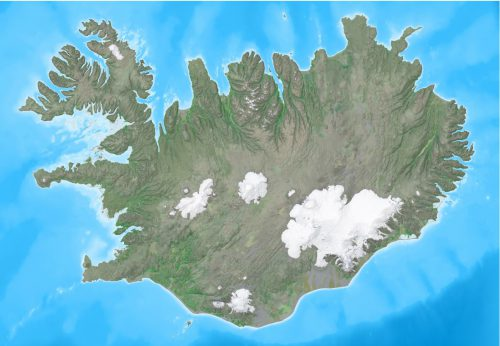
\includegraphics[width=0.21\textwidth, clip, trim=0 0 0 1mm]{Map}};
            \node[anchor=north] (photo) at ($(plan.south west)!0.5!(sectionTitle.south west |- plan.south)-(0,1mm)$) {
                \ifCompileWithPhotos%
                    \IfImageCanBeIncluded{#2}{%
                        \includegraphics[width=0.85\textwidth]{#2}
                    }{%
                        \includegraphics[width=0.75\textwidth]{example-image-a}
                    }
                \else
                    \includegraphics[width=0.75\textwidth]{example-image-a}
                \fi
            };
            \node[text depth=0.5ex, below = 2mm of photo.south east, anchor=north east, xshift=-2pt]{#3};
            \ifthenelse{\isempty{#1}}{}%
            {
                \begin{scope}[x={($ (plan.south east) - (plan.south west) $ )},y={( $ (plan.north west) - (plan.south west)$ )}, shift={(plan.south west)}]
                    %\draw[help lines,xstep=.1,ystep=.1] (0,0) grid (1,1);
                    \node[anchor=south, inner sep=0] at (#1) {
\includegraphics[width=2mm]{Pin}};
                \end{scope}
            }
            \ifCompileWithPhotos
                \IfImageCanBeIncluded{#2}{%
                    \node[rotate=90, anchor=west, font=\ssmall] at ($(current page.south east)+(-2mm,1mm)$) {{\raisebox{-2mm}{\Large\textcopyright}} Photo: All rights are reserved};
                }{}
            \fi
        \end{tikzpicture}
    }
    %Add a link to table of content on frames with a footline
    \addtobeamertemplate{footline}{}{%
        \ifAddLinkToTOC%
            \begin{tikzpicture}[remember picture,overlay]
                %xelatex needs \XeTeXLinkBox, won't create a link unless it
                %finds text --- rules don't work without \XeTeXLinkBox.
                %Still builds correctly with pdflatex and lualatex
                \node[anchor=south east, inner sep=2pt] at (current page.south east) {\hyperlink{toc}{\XeTeXLinkBox{
\includegraphics[width=3mm]{TOC}}}};
            \end{tikzpicture}%
        \fi%
    }%
}

\makeatletter
\AtBeginSection[]% <- Empty optional argument, do nothing for \section*
{%
    \ifnum\beamer@tocsectionnumber>0%
        \begin{frame}[plain, noframenumbering]{}
             \sectionpage
        \end{frame}
    \fi
}
\makeatother

%Append code to put third CSC logo on titlepage
\appto\titlepage{%
    \begin{tikzpicture}[remember picture, overlay]
        \node[anchor=south] at (current page.south) {
\includegraphics[width=25mm]{LogoCSC}};
    \end{tikzpicture}
}

%===============================================================%
\title{Introduction to Bash scripting language}
\author{Alessandro Sciarra \texorpdfstring{\\}{} {\tiny Z02~--~Software Development Center}}
\institute{Organised by the CSC Frankfurt}
\titlegraphic{
\includegraphics[width=20mm]{LogoCRC}}
\titlepagelogo{
\includegraphics[width=20mm]{LogoGoethe}}
%===============================================================%


%===================%
\subtitle{Day 1}
\date{07.10.2019}
%===================%

\begin{document}
    %-------------------------------%
%  Author: Alessandro Sciarra   %
%    Date: 5 Jun 2019           %
%-------------------------------%

%~~~~~~~~~~~~~~~~~~~~~~~~~~~~~~~~~~~~~~~~~~~~%
\begin{frame}[plain,noframenumbering]
    \titlepage
\end{frame}
%~~~~~~~~~~~~~~~~~~~~~~~~~~~~~~~~~~~~~~~~~~~~%
\begin{frame}[plain,noframenumbering]{Topics of the day}
    \medskip
    \begin{columns}[t]
        \begin{column}{.45\textwidth}
            \hspace*{4mm}
            \begin{minipage}[t][0.6\textheight]{\textwidth}
                \tableofcontents[sections={1-6}]
            \end{minipage}
        \end{column}
        \begin{column}{.45\textwidth}
            \begin{minipage}[t][0.6\textheight]{\textwidth}
                \tableofcontents[sections={7-}]
            \end{minipage}
        \end{column}
    \end{columns}
\end{frame}
%~~~~~~~~~~~~~~~~~~~~~~~~~~~~~~~~~~~~~~~~~~~~%

    \addSection{Inception and Philosophy}{example-image-a}{distribution image}
    %-------------------------------%
%  Author: Alessandro Sciarra   %
%    Date: 21 Sep 2020          %
%-------------------------------%

%~~~~~~~~~~~~~~~~~~~~~~~~~~~~~~~~~~~~~~~~~~~~%
\begin{frame}{An often mistreated language}
    \begin{itemize}
        \item Everybody uses Bash
        \item It is easy to know a bit of many commands\tikzmark{arrowfrom}
        \item Not so many Bash users (have time to) go deeply into the details
    \end{itemize}
    \begin{varblock}{alerted}[0.8\textwidth]{The nature of Bash}
        \PQ{As with many tools, it is common to just get stuff working, no matter how}
    \end{varblock}
    %\vspace{2mm}
    \begin{overlayarea}{\textwidth}{0.6\textheight}
        \begin{varblock*}{example}[0.8\textwidth]{Important aspects to \textbf{always} keep in mind}<only@2>
            $\circ\;$Use a clear, readable layout\\
            $\circ\;$Avoid unnecessary commands\\
            $\circ\;$A small, trivial script today might become large and complex tomorrow
        \end{varblock*}
        \begin{tikzpicture}[remember picture, overlay]
            \path[to, PT] (arrowfrom) ++(5mm,0) edge[out=20, in=60, looseness=3]  ++(22mm, -11mm) coordinate (arrival);
            \path[to, visible on=<2>, PS] (arrival)   ++(-53mm,-18mm) edge[out=200, in=150, looseness=2] ++(0mm, -13mm);
        \end{tikzpicture}
        \begin{varblock}{quote}[0.9\textwidth]{Before you get too excited}[Greg's Wiki]<only@3>
            It is key that you remember, Bash is a tool, a single tool in a huge toolbox of programs.
            Bash alone will only let you do basic things with files and other programs.
            You will need to understand all the other tools in the toolbox of your system.
            This knowledge is vast and will come slowly, it is important that you take the time to learn them well rather than try to get the basic idea of most and break a leg tomorrow (or more likely, your music archive or collection of family pictures).
        \end{varblock}
    \end{overlayarea}
\end{frame}
%~~~~~~~~~~~~~~~~~~~~~~~~~~~~~~~~~~~~~~~~~~~~%
\begin{frame}[fragile]{Using Bash}
    \vspace{-2mm}
    \begin{description}
        \item[Bash in interactive mode:] A prompt and a command line
        \item[Bash in non-interactive mode:] Executing scripts
    \end{description}
    \begin{varblock*}{}[0.7\textwidth]{The prompt}
        \texttt{\PQ{cool-prompt}\PT{\$}} $\;\leftarrow\;$ shell compatible with the Bourne shell\\
        \texttt{\PQ{cool-prompt}\PT{\%}} $\;\leftarrow\;$ C-shell (which is not covered here)\\
        \texttt{\PQ{cool-prompt}\PT{\#}} $\;\leftarrow\;$ shell run as superuser (root)
    \end{varblock*}
    \begin{onlyenv}<2>
        \begin{lstlisting}[style=MyBash, aboveskip=5mm]
            $ man man      # Learn how to use and read the manual@|$^\star$|@
            $ man apropos
            $ help         # Get help for builtin commands
            $ help echo
        \end{lstlisting}
        \medskip
        \hfill {\scriptsize $^\star\;$Use \keystroke{Q} to quit the manual}\hspace{1cm}
    \end{onlyenv}
    \begin{varblock*}{example}[0.7\textwidth]{Manual \textbf{SYNOPSIS}}<only@3>
        \footnotesize
        \begin{tabular}{@{\qquad}ll}
            \textbf{bold text}                       &    type exactly as shown.\\
            \underline{italic} \underline{text}      & replace with appropriate argument.\\
            {}[-abc]                                 & any or all arguments within [ ] are optional.\\
            -a|-b                                    & options delimited by | cannot be used together.\\
            \underline{\smash{argument}} ...         & argument is repeatable.\\
            {}[~\underline{\smash{expression}}~] ... & entire expression within [ ] is repeatable.\\
        \end{tabular}
    \end{varblock*}
\end{frame}
%~~~~~~~~~~~~~~~~~~~~~~~~~~~~~~~~~~~~~~~~~~~~%
\begin{frame}{The goal of the day}
    \begin{itemize}
        \item \alert<2>{Arguments}\tikzmark{ptA}
        \item \alert<2>{Quotes}\tikzmark{ptB}
        \item Shell parameters
        \item Special variables (e.g. \bash{IFS})
        \item Shell expansion
              \begin{itemize}
                  \item Brace expansion
                  \item Parameters expansion\tikzmark{ptC}
                  \item \ldots
                  \item \alert<2>{Word splitting}
                  \item Filename expansion
              \end{itemize}
        \item Globbing
        %\item Regular expressions
        %\item Brace expressions
        %\item \bash|if|, \bash|test| and \bash{[[}
    \end{itemize}
    \begin{tikzpicture}[remember picture, overlay, scope on=<2>]
        \coordinate (remark) at ($(ptA)!0.5!(ptC)+(25mm,0)$);
        \node[anchor=west, starburst, minimum height=3cm, starburst point height=8mm, line width=1mm,
              draw=PT, fill=yellow, fill opacity=0.3, text opacity=1, text=PQ,
              visible on=<2>, fill on=<2>, text on=<2>] (cloud) at ($(remark)+(3mm,0)$) {The Bash inner core};
        \node[below = 25mm of cloud, text=PP, rounded corners=3pt, draw=PB, thick, inner sep=2mm] (learn) {Take your time and learn them well!};
        \draw[to, shorter={2mm}{1mm}] (cloud.south) -- (learn);
    \end{tikzpicture}
    \FrameRemark<2>{\PQ{\textbf{Disclaimer:}} \alert{Some slides will unavoidably refer to later material. Hopefully, everything will be clarified at the end of the day and, for sure, by Friday!}}
\end{frame}
%~~~~~~~~~~~~~~~~~~~~~~~~~~~~~~~~~~~~~~~~~~~~%

    \addSection{Commands and arguments}[0.5,0.5]{example-image-b}{image}
    %-------------------------------%
%  Author: Alessandro Sciarra   %
%    Date: 17 Jun 2019          %
%-------------------------------%

%~~~~~~~~~~~~~~~~~~~~~~~~~~~~~~~~~~~~~~~~~~~~%
\begin{frame}[fragile]{How does Bash interpret a line of code?}
    \begin{itemize}
        \item Bash divides each line into words that are demarcated by a \textbf{whitespace character}$^\star$.\tikzmark{whitespace}
        \item \alert{The first word} of the line is the name of \alert{the command} to be executed.
        \item \PP{All the remaining words} become \PP{arguments} to that command (options, filenames, etc.).
    \end{itemize}
    \begin{lstlisting}[style=MyBash, showspaces=true, aboveskip=1mm]
         $@|~|@command arg1 arg2   arg3       arg4
         $@|~|@command arg1 arg2 arg3 arg4
    \end{lstlisting}
    \vspace{2mm}
    \begin{varblock}{alerted}[0.75\textwidth]{}
        \PQ{The amount of whitespace between arguments does not matter!}
    \end{varblock}
    \begin{lstlisting}[style=MyBash, aboveskip=2mm]
        $ echo I am Clark Kent
        |+I am Clark Kent+|                        # <- Same output
        $ echo I    am  Clark         Kent
        |+I am Clark Kent+|                        # <- as here!
    \end{lstlisting}
    \FrameRemark{$^\star$There are a few advanced cases, such as commands that span multiple lines, that have slightly different rules.}
    \begin{tikzpicture}[remember picture, overlay]
        \node[above= 8mm of whitespace, anchor=east, font=\scriptsize, xshift=4pt] (label) {Spaces and Tabs};
        \path[to] (label) edge[out=0, in=0, looseness=1.8] (whitespace);
    \end{tikzpicture}
\end{frame}
%~~~~~~~~~~~~~~~~~~~~~~~~~~~~~~~~~~~~~~~~~~~~%
\begin{frame}[fragile]{The first hurdle: spaces}{How can a so innocent, invisible character hurt me? ...well...}
    \vspace{-3mm}
    \begin{itemize}
        \item To a shell, whitespace is incredibly important
        \item Don't be fooled into thinking a space or tab more or less won't make much of a difference
        \item  Whitespace is \textbf{vital} to allowing your shell to understand you
    \end{itemize}
    \begin{lstlisting}[style=MyBash, aboveskip=4mm]
        $ ls -1
        |+The secret voice.mp3
        secret+|
        $ rm The secret voice.mp3  # rm gets 3 arguments, not 1!
        |+rm: cannot remove 'The': No such file or directory+|
        |+rm: cannot remove 'voice.mp3': No such file or directory+|
        $ ls
        |+The secret voice.mp3+|       # Where's your file 'secret'!?
    \end{lstlisting}
    \centerline{\ssmall \bash|ls| and \bash|rm| are commands to list the present working directory content and to remove files, respectively.}
    \vspace{-3mm}
    \begin{overlayarea}{\textwidth}{0.3\textheight}
        \begin{varblock}{example}[0.5\textwidth]{}<only@1>
            We will deepen into \PS{Word splitting} later!
        \end{varblock}
        \begin{varblock}{}[0.9\textwidth]{Side remark}<only@2>
            \PB{Whitespaces in filenames} should be avoided and \PB{replaced by underscores}. Everything would be much easier. But they are allowed... so deal with it!
        \end{varblock}
    \end{overlayarea}
\end{frame}
%~~~~~~~~~~~~~~~~~~~~~~~~~~~~~~~~~~~~~~~~~~~~%
    \addSection{Strings and type of commands}[0.5,0.5]{example-image-b}{image}
    %-------------------------------%
%  Author: Alessandro Sciarra   %
%    Date: 23 Sep 2020          %
%-------------------------------%

%~~~~~~~~~~~~~~~~~~~~~~~~~~~~~~~~~~~~~~~~~~~~%
\begin{frame}[noframenumbering, plain]{After all it is simple...}
    \centering
    
\includegraphics[width=0.9\textwidth]{ToyStory}
\end{frame}
%~~~~~~~~~~~~~~~~~~~~~~~~~~~~~~~~~~~~~~~~~~~~%
\begin{frame}{Strings, strings everywhere}
    \vspace{-3mm}
    The term string refers to a sequence of characters which is treated as a single unit:
    \begin{itemize}
        \item The command's name is a string
        \item Each argument of a command is a string
        \item Variable names are strings
        \item The contents of variables are strings as well
        \item A filename is a string
        \item Most files contain strings
    \end{itemize}
    \begin{varblock}{alerted}[0.7\textwidth]{Strings do not have any intrinsic meaning}
        Their meaning is defined by how and where they are used. 
    \end{varblock}
    \begin{varblock}{}[0.85\textwidth]{We have \textbf{all} the responsibility}
        We need to be sure everything that needs to be separated is separated properly, and everything that needs to stay together stays together properly!
    \end{varblock}
    \FrameRemark{I will loosely use the term \textbf{string} throughout the lecture, mostly referring to a portion of text contained in a variable}
\end{frame}
%~~~~~~~~~~~~~~~~~~~~~~~~~~~~~~~~~~~~~~~~~~~~%
\begin{frame}<1>[fragile, label=CommandsTypes]{Types of commands}
    \only<1>{\framesubtitle{There are basically 5 different classes of commands}}
    \only<2->{\framesubtitle{}}
    \begin{onlyenv}<1>
        \begin{center}
            \begin{tikzpicture}
                \node[minimum size=5cm, circle, draw, thin] (O) at (0,0) {};
                \foreach \l [count=\li, evaluate=\li as \angle using int(\li*72)] in {Aliases, Functions, Builtins, Keywords, Executables}{
                    \node[cloud, draw, text=PB, fill=PP!20, aspect=2] at (O.\angle) {\l};
                }
            \end{tikzpicture}
        \end{center}
    \end{onlyenv}
    \vspace{-6mm}
    \begin{onlyenv}<2->
        \setlength{\columnsep}{-5mm}
        \begin{multicols}{5}
            \begin{enumerate}
                \item \tc<2>{PP}{Aliases}
                \item \tc<3>{PP}{Functions}
                \item \tc<4-6>{PP}{Builtins}
                \item \tc<7>{PP}{Keywords}
                \item \tc<8>{PP}{Executables}
            \end{enumerate}
        \end{multicols}
    \end{onlyenv}
    \vspace{-3mm}
    \begin{overlayarea}{\textwidth}{0.7\textheight}
        \begin{onlyenv}<2>
            \begin{itemize}
                \item An alias is a rudimentary way of shortening a command
                \item \PP{It is a word that is mapped to a certain string}
                \item They are only used in \textbf{interactive} shells and \textbf{not} in scripts
                \item They are limited in power; the replacement only happens in the first word
                \item An alias should effectively not do more than change the default options of a command
                \item For more complex tasks and more flexibility, use a function
            \end{itemize}
            \begin{lstlisting}[style=MyBash]
                $ help alias
                |+alias: alias [-p] [name[=value] ... ]+|
                |+    Define or display aliases.       +|

                # [More information]

                $ alias ls='ls --color=auto'
                $ ls  # The command executed is, instead:  ls --color=auto
            \end{lstlisting}
            \FrameRemark{Bash stores the values of aliases in an array called \bash|BASH_ALIASES|}
        \end{onlyenv}
        \begin{onlyenv}<3>
            {\Large
            \begin{varblock}{alerted}[0.7\textwidth]{Functions are tricky!}
                They will be covered in depth later in the course
            \end{varblock}}
            \bigskip
            For the moment, a few hints:
            \begin{itemize}
                \item Functions in Bash are more powerful than aliases and the are often the way to go
                \item Unlike aliases, they can be used in scripts, i.e. in non-interactive mode
                \item A function contains shell commands, and acts very much like a small script
                \item They can even take arguments and create local variables
                \item When a function is called, the commands in it are executed
            \end{itemize}
        \end{onlyenv}
        \begin{onlyenv}<4-6>
            \begin{itemize}
                \item Builtins are basic commands that Bash has built into it
                \item They can be thought as functions that are already provided
                \item We will learn about (or at least mention) \tc<5>{PP}{most of them}
                \item Keywords which are provided as builtins are nevertheless highlighted as \tc<6>{keywords-color}{keywords}
            \end{itemize}
            \begin{onlyenv}<4>
                \begin{lstlisting}[style=MyBash, numbers=none, keywordstyle=\color{builtins-color},]
                   :         complete   export    let        shift     umask  
                   .         compgen    false     local      shopt     unalias
                   [         continue   fc        logout     source    unset  
                   alias     declare    fg        popd       suspend   until  
                   bg        dirs       getopts   printf     test      wait   
                   bind      disown     hash      pushd      times     while  
                   break     echo       help      pwd        trap      
                   builtin   enable     history   read       true      
                   case      eval       if        readonly   type      
                   cd        exec       jobs      return     typeset   
                   command   exit       kill      set        ulimit    
                \end{lstlisting}
            \end{onlyenv}
            \begin{onlyenv}<5>
                \begin{lstlisting}[style=MyBash, numbers=none, deleteemph={[5]:,.,[,alias, bg, bind, break, case, cd, complete, compgen, continue, declare, dirs, disown, echo, eval, exec, exit, export,false, fg, help, if, jobs, kill, let, local, popd, printf, pushd, pwd, read, readonly, return, set, shift, shopt, source, test, trap, true, unalias, unset, until, wait, while}, emph={[7]:,.,[,alias, bg, bind, break, case, cd, complete, compgen, continue, declare, dirs, disown, echo, eval, exec, exit, export,false, fg, help, if, jobs, kill, let, local, popd, printf, pushd, pwd, read, readonly, return, set, shift, shopt, source, test, trap, true, unalias, unset, until, wait, while}, emphstyle={[7]\color{PP}}]
                   :         complete   export    let        shift     umask  
                   .         compgen    false     local      shopt     unalias
                   [         continue   fc        logout     source    unset  
                   alias     declare    fg        popd       suspend   until  
                   bg        dirs       getopts   printf     test      wait   
                   bind      disown     hash      pushd      times     while  
                   break     echo       help      pwd        trap      
                   builtin   enable     history   read       true      
                   case      eval       if        readonly   type      
                   cd        exec       jobs      return     typeset   
                   command   exit       kill      set        ulimit    
                \end{lstlisting}
            \end{onlyenv}
            \begin{onlyenv}<6>
                \begin{lstlisting}[style=MyBash, numbers=none]
                   :         complete   export    let        shift     umask  
                   .         compgen    false     local      shopt     unalias
                   [         continue   fc        logout     source    unset  
                   alias     declare    fg        popd       suspend   until  
                   bg        dirs       getopts   printf     test      wait   
                   bind      disown     hash      pushd      times     while  
                   break     echo       help      pwd        trap      
                   builtin   enable     history   read       true      
                   case      eval       if        readonly   type      
                   cd        exec       jobs      return     typeset   
                   command   exit       kill      set        ulimit    
                \end{lstlisting}
            \end{onlyenv}
        \end{onlyenv}
        \begin{onlyenv}<7>
            \begin{varblock}{alerted}[0.75\textwidth]{}
                Keywords are like builtins, but \alert{special parsing rules apply to them}
            \end{varblock}
            \begin{itemize}
                \item Flow control constructs is achieved thanks to keywords
                \item We will explore all of them in detail \Remark[2mm]{except \bash|coproc|}
            \end{itemize}
            \begin{lstlisting}[style=MyBash, numbers=none]
                if     elif   esac     while   done      time   !    coproc
                then   fi     for      until   in        {      [[
                else   case   select   do      function  }      ]]
            \end{lstlisting}
            \bigskip
            For example:
            \medskip
            \begin{lstlisting}[style=MyBash]
                $ [ a < b ]   # Oops, < means here input redirection!
                |+-bash: b: No such file or directory+|
                $ [[ a < b ]] # The meaning of < changes within [[ ]]
            \end{lstlisting}
        \end{onlyenv}
        \begin{onlyenv}<8>
            \begin{itemize}
                \item Executables are the last type of command that Bash can execute
                \item They are also known as external commands or applications
                \item They are typically invoked by their name, on the constraint that Bash is able to find them
                \item When a command is specified without a file path and it is \alert{not an alias, a function, a builtin or a keyword}, Bash searches through the directories contained in the variable \bash|PATH|
                \item The search is done from left to right and the first executable found is run
            \end{itemize}
            \begin{lstlisting}[style=MyBash]
                $ ls /home/sciarra/.local/bin
                |+...   g++   ...+| # Version 8.3.0
                $ ls /usr/bin
                |+...   g++   ...+| # Version 5.4.0
                $ echo ${PATH}
                |+/home/sciarra/.local/bin:/usr/bin:/bin+|
                $ g++ -dumpversion
                |+8.3.0+|
            \end{lstlisting}
        \end{onlyenv}
    \end{overlayarea}
\end{frame}
%~~~~~~~~~~~~~~~~~~~~~~~~~~~~~~~~~~~~~~~~~~~~%
\againframe<2>{CommandsTypes}
%~~~~~~~~~~~~~~~~~~~~~~~~~~~~~~~~~~~~~~~~~~~~%
\againframe<3>{CommandsTypes}
%~~~~~~~~~~~~~~~~~~~~~~~~~~~~~~~~~~~~~~~~~~~~%
\againframe<4-6>{CommandsTypes}
%~~~~~~~~~~~~~~~~~~~~~~~~~~~~~~~~~~~~~~~~~~~~%
\againframe<7>{CommandsTypes}
%~~~~~~~~~~~~~~~~~~~~~~~~~~~~~~~~~~~~~~~~~~~~%
\againframe<8>{CommandsTypes}
%~~~~~~~~~~~~~~~~~~~~~~~~~~~~~~~~~~~~~~~~~~~~%
\begin{frame}[fragile]{Bash scripts}
    \vspace{-6mm}
    \begin{itemize}
        \item A script is a sequence of Bash commands in a file
        \item The commands are read and processed \PP{in order}
        \item A new command is processed after the previous has \PP{ended} \Remark{unless differently required}
        \item The first line of a script should be reserved for an \textbf{interpret directive} also called \alert{hashbang} or \alert{shebang}.
              This is used when the kernel executes a non-binary file.
              Use one of the two following alternatives: \\
              \begin{center}
                  \begin{tikzpicture}
                      \node[fill=background-color, inner sep=1mm, font=\scriptsize] (shebangA) {\bash|#!/bin/bash|};
                      \node[fill=background-color, inner sep=1mm, font=\scriptsize, right = 3cm of shebangA] (shebangB) {\bash|#!/usr/bin/env bash|};
                      \draw[to, shorter={2mm}{2mm}] (shebangA) -- node[midway, above=-1pt, font=\tiny] {or, preferably,} (shebangB);
                  \end{tikzpicture}
                  \par{\ssmall The right directive has the benefit of looking for whatever the default version of the program is in your current \textbf{env}ironment (i.e. in \bash|PATH|).}
              \end{center}
        \item<only@1> Please, \alert{do not use} \,\raisebox{0.1em}{\fbox{\ssmall\bash|#!/bin/sh|}}\, as shebang, even if you might see it around on the web!
        \item<only@1> Avoid giving your scripts a \textbf{.sh} extension. Do not use one or use \alert{\textbf{.bash}}!
        \item<only@2> Execute the script in either of the following ways:
    \end{itemize}
    \begin{varblock}{alerted}[0.75\textwidth]{\textbf{Sh is NOT Bash!}}<only@1>
        \textbf{Bash} itself is a \textbf{sh-compatible} shell however, the opposite is not true!
    \end{varblock}
    \begin{onlyenv}<2>
        \begin{lstlisting}[style=MyBash]
            $ bash myscript   #The shebang is treated as a comment!
        \end{lstlisting}
        \centerline{or}
        \begin{lstlisting}[style=MyBash]
            $ chmod +x myscript  # Make the file executable
            $ ./myscript         # Execute it, the shebang is used!
        \end{lstlisting}
    \end{onlyenv}
\end{frame}
%~~~~~~~~~~~~~~~~~~~~~~~~~~~~~~~~~~~~~~~~~~~~%



    \addSection{Quoting and Special characters}[0.5,0.5]{example-image-b}{image}
    %-------------------------------%
%  Author: Alessandro Sciarra   %
%    Date: 19 Jun 2019          %
%-------------------------------%

%~~~~~~~~~~~~~~~~~~~~~~~~~~~~~~~~~~~~~~~~~~~~%
\begin{frame}[label={Quotes}]{Types of quoting}
    \vspace{-4mm}
    \begin{description}
        \item[Single quotes] Everything inside single quotes becomes a literal string\\[-0.3em]
                             {~\tiny\{The only character that you can't safely enclose in single quotes is a single quote.\}}
        \item[Double quotes] Performed actions:
                             \begin{itemize}
                                 \item Every substitution that begins with a dollar sign \texttt{\$}
                                 \item Backslash escaping
                                 \item \tc{Gray!30}{The legacy \texttt{\textasciigrave\ldots\textasciigrave} (backticks) command substitution}
                             \end{itemize}
                             \alert{No word splitting or filename expansion is performed!}
        \item[Backticks] \tc{Gray!30}{\texttt{\textasciigrave\ldots\textasciigrave} is the legacy command substitution syntax}\\
                         \alert{Deprecated in favor of \texttt{\$(\ldots)}}
        \item[Backslash] Putting \texttt{\textbackslash} in front of a metacharacter removes its special meaning\\[-0.3em]
                         {~\tiny\{This works inside double quotes, or in the absence of quotes. It does not work inside single quotes.\}} 
        \item[\texttt{\$'\ldots'}] A Bash extension that prevents everything except backslash escaping\\
                                   It also allows special backslash escape sequences like \texttt{\textbackslash{}n} for newline%, \t for tab, and \xnn for bytes specified in hexadecimal. 
        \item[\texttt{\$"\ldots"}] Bash extension used for \URL[PP]{http://mywiki.wooledge.org/BashFAQ/098}{localisation support}, not covered here
    \end{description}
    \FrameRemark{This is the short story. The verbose version is available at the end of \URL[PB]{http://mywiki.wooledge.org/Quotes}{this page}.}
\end{frame}
%~~~~~~~~~~~~~~~~~~~~~~~~~~~~~~~~~~~~~~~~~~~~%
\begin{frame}[fragile]{Examples about quoting}
    \begin{onlyenv}<1>
        \begin{lstlisting}[style=MyBash, style=oddnumbers]
            $ echo I    am  Clark       Kent
            |+I am Clark Kent+|
            $ echo I"    "am"  "Clark"       "Kent        # Not nice
            |+I    am  Clark         Kent+|
            $ echo I\ \ \ \ am\ \ Clark\ \ \ \ \ \ \ Kent # Really!?
            |+I    am  Clark         Kent+|
            $ echo 'I    am  Clark       Kent'
            |+I    am  Clark       Kent+|
            $ echo "I    am  Clark       Kent"
            |+I    am  Clark         Kent+|
        \end{lstlisting}
        \centerline{\tiny }
        \medskip
        \begin{lstlisting}[style=MyBash, style=oddnumbers, firstnumber=10]
            $ echo 'PATH contains ${PATH}'
            |+PATH contains ${PATH}+|
            $ echo "PATH contains ${PATH}"
            |+PATH contains /home/sciarra/.local/bin:/usr/bin:/bin+|
            $ echo "PATH contains \${PATH}"
            |+PATH contains ${PATH}+|
        \end{lstlisting}
    \end{onlyenv}
    \begin{onlyenv}<2>
        \renewcommand\thelstnumber{\ifnum\value{lstnumber}=11\relax\else\arabic{lstnumber}\fi}
        \begin{lstlisting}[style=MyBash, style=oddnumbers, firstnumber=16]
            $ ls *.tex
            |+Day_1.tex   Day_2.tex   Day_3.tex+|
            $ ls '*.tex'
            |+ls: cannot access '*.tex': No such file or directory+|
            $ ls "*.tex"
            |+ls: cannot access '*.tex': No such file or directory+|
            $ echo "Hello\nWorld"
            Hello\nWorld
            $ echo $'Hello\nWorld'
            Hello
            @|\renewcommand\thelstnumber{}|@World
        \end{lstlisting}
    \end{onlyenv}
    \begin{varblock}{alerted}[0.9\textwidth]{I'm Too Lazy to Read, Just Tell Me What to Do}<2>
        \begin{lstlisting}[style=MyBash, numbers=none, belowskip=-6mm,aboveskip=2mm]
            $ cp $file $destination         # WRONG
            $ cp -- "$file" "$destination"  # Right
        \end{lstlisting}
        When in doubt, \textbf{double-quote every expansion} in your shell commands.\\
        Generally use \textbf{double quotes} unless it makes more sense to use single quotes.
    \end{varblock}
\end{frame}
%~~~~~~~~~~~~~~~~~~~~~~~~~~~~~~~~~~~~~~~~~~~~%
\begin{frame}[fragile]{Special characters}{Just a brief overview}
    \vspace{-6mm}
    \begin{columns}
        \begin{column}{\dimexpr\paperwidth-10mm}
            \begin{description}[\texttt{>  >>  <}]
                \setlength{\itemsep}{1mm}
                \item<only@1>[\texttt{\textvisiblespace}]
                    A \alert{white}\tikzmark{whitespace}\alert{space} is used by Bash to determine where words begin and end \\
                    The first word is the command name and additional words become arguments
                \item<only@1>[\texttt{\$}]
                    It introduces various types of \alert{expansion}:
                    \begin{tabular}{ll}
                        \PB{$\bullet\;$} parameter expansion   & \texttt{\$\{var\}}          \\
                        \PB{$\bullet\;$} command substitution  & \texttt{\$(command)}      \\
                        \PB{$\bullet\;$} arithmetic expansion  & \texttt{\$((expression))} \\
                    \end{tabular}
                \item<only@1>[\texttt{' '}] \alert{Single quotes}\tikzmark{curlyStart}
                \item<only@1>[\texttt{" "}] \alert{Double quotes}
                \item<only@1>[\texttt{\textbackslash}] \alert{Escape symbol}\tikzmark{curlyEnd}
                \item<only@1>[\texttt{\#}]
                    It introduced a \alert{comment} that extends to the end of the line. \\
                    Text after it is ignored by the shell. {~\tiny\{In single and double quotes, \texttt{\#} is just a \texttt{\#}.\}}
                \item<only@2>[\texttt{=}]
                    The \alert{assignment} symbol is used to assign a value to a variable \\
                    Whitespace is not allowed on either side of the \texttt{=} character
                \item<only@2>[\texttt{[[ ]]}]
                    This \alert{testing keyword} allows to evaluate a conditional expression \\
                    to determine whether it is ``true'' or ``false''
                \item<only@2>[\texttt{!}]
                    The \alert{negate keyword} reverses a test or an exit status
                \item<only@2>[\texttt{>  >>  <}]
                    \alert{Redirection} of a command's output or input to a file
                \item<only@2>[\texttt{|}]
                    The \alert{pipeline} sends the output from one command to the input of another command
                \item<only@2>[\texttt{;}]
                    \alert{Command separator} of multiple commands that are on the same line 
                \item<only@2>[\texttt{\{ \}}]
                    An \alert{inline group} allows to treat multiple commands as if they were one command
                    Convenient to be uses when Bash syntax requires only one command
                \item<only@2>[\texttt{( )}]
                    Another way to group commands, but in a \alert{subshell group} \\
                    However, commands in \texttt{( )} are executed in a subshell (a new process) \\
                    and this is often the way to avoid side effects on the current shell
                \item<only@3-4>[\texttt{(( ))}]
                     Within an \alert{arithmetic expression}, mathematical oper\tikzmark{operators}ators are used for calculations \\
                     They can be used for\\
                     \begin{tabular}{ll}
                        \PB{$\bullet\;$} variable assignments   & \texttt{(( a = 1 + 4 ))}  \\
                        \PB{$\bullet\;$} tests evaluation       & \texttt{(( a < b ))}      \\
                    \end{tabular}
                \item<only@3-4>[\texttt{\$(( ))}]
                    Comparable to \texttt{(( ))}, but the expression is replaced with the result of its evaluation
                \item<only@3-4>[\texttt{*  ?}]
                    \alert{Globbing} characters are wildcards which match parts of filenames
                \item<only@3-4>[\texttt{\~}]
                    The tilde is a representation of a \alert{home directory}\\
                    When alone or followed by a \texttt{/}, it means the current user's home directory \\
                    Otherwise, a username must be specified: \bash|ls ~john/|
                \item<only@3-4>[\texttt{\&}]
                    When used at the end of a command, run the command in the \alert{background} \\
                    The shell does not wait for it to complete
            \end{description}
        \end{column}
    \end{columns}
    \begin{varblock}{}[0.9\textwidth]{More details later}<only@4>
        \PB{We will come back to these special instructions with details and examples} 
    \end{varblock}
    \begin{tikzpicture}[remember picture, overlay]
        \begin{scope}[scope on=<1>]
            \node[font=\ssmall, above = 4mm of whitespace, anchor=west, xshift=1cm] (ws) {\{a space, tab, newline, carriage return, vertical tab or form feed\}};
            \path[to] (ws.west) edge[out=180, in=90] ([yshift=2mm]whitespace);
            \draw[very thick, decorate, decoration={brace,amplitude=6pt}] (curlyStart -| curlyEnd) ++(5mm,1mm) -- ($(curlyEnd)+(5mm,-1mm)$) 
                  node[midway, right=3mm, text width=25mm, align=center] {Already discussed on slide~\ref{Quotes}};
        \end{scope}
        \begin{scope}[scope on=<3-4>]
            \node[font=\ssmall, above = 4mm of operators, anchor=west, xshift=1cm] (ops) {the 4 characters\,\,\fbox{\texttt{+~~~-~~~*~~~/}}};
            \path[to] (ops.west) edge[out=180, in=90] ([yshift=2mm]operators);
        \end{scope}
    \end{tikzpicture}
\end{frame}
%~~~~~~~~~~~~~~~~~~~~~~~~~~~~~~~~~~~~~~~~~~~~%
\begin{frame}{Deprecated special character}
    \begin{columns}
        \begin{column}{\dimexpr\paperwidth-10mm}
            \begin{description}[\texttt{>  >>  <}]
                \setlength{\itemsep}{1mm}
                \color{Gray!30}
                \item[\texttt{\textasciigrave\ \textasciigrave}]
                    Command substitution - \alert{use \texttt{\$( )} instead}\tikzmark{backticks}
                \item[\texttt{[ ]}]
                    An alias for the old test command\\
                    Commonly used in POSIX shell scripts\\
                    \alert{Lacks many features of \texttt{[[ ]]}}\tikzmark{test}
                \item[\texttt{\$[ ]}]
                    Arithmetic expression - \alert{use \texttt{\$(( ))} instead} \\
                    Simply do not use it, it dates back to 1990s!!!
            \end{description}
        \end{column}
    \end{columns}
    \bigskip
    \begin{varblock}{}[0.9\textwidth]{Legacy code and portability}
        Unless you have very special requirement, try to stick to modern Bash features!
    \end{varblock}
    \begin{tikzpicture}[remember picture, overlay, every node/.style={anchor=east, xshift=-1cm, font=\ssmall}]
        \node at (current page.east |- backticks) (A) {\URL[PB]{http://mywiki.wooledge.org/BashFAQ/082}{Advance reading}};
        \node at (current page.east |- test) (B) {\URL[PB]{http://mywiki.wooledge.org/BashFAQ/031}{Advanced reading}};
        \path[from, shorter={5mm}{5mm}, thin, Gray!30] (backticks) edge (A) (test) edge (B);
    \end{tikzpicture}
    \FrameRemark{At the end of the lecture, you might come back to \URL[PP]{https://wiki.bash-hackers.org/scripting/obsolete}{this page} and read about obsolete features!}
\end{frame}
%~~~~~~~~~~~~~~~~~~~~~~~~~~~~~~~~~~~~~~~~~~~~%

    \addSection{Variables and special parameters}[0.5,0.5]{example-image-b}{image}
    %-------------------------------%
%  Author: Alessandro Sciarra   %
%    Date: 23 Sep 2020          %
%-------------------------------%

%~~~~~~~~~~~~~~~~~~~~~~~~~~~~~~~~~~~~~~~~~~~~%
\begin{frame}[fragile]{The first building block}
    Parameters come in two flavours:
    \begin{itemize}
        \item Variables (i.e. parameters with a name)\\[0.1em]
              {\scriptsize $\to$ Created and updated by the user \\[-0.5em] $\to$ Available in the environment}
        \item {\color{Gray!50}Special parameters (later)\tikzmark{origin}\\
              {\scriptsize $\to$ Read-only and pre-set by Bash}}
    \end{itemize}
    \begin{tikzpicture}[remember picture, overlay, line join=round]
        \pgfmathsetmacro{\cubex}{1}
        \pgfmathsetmacro{\cubey}{1}
        \pgfmathsetmacro{\cubez}{1}
        \coordinate (O) at ([xshift=30mm]origin);
        \draw[PS, fill=PS!40] (O) ++(\cubex,\cubey,0) -- ++(0,0,-\cubez) -- ++(0,-\cubey,0) -- ++(0,0,\cubez) -- cycle;
        \draw[PS, fill=PS!10] (O) ++(\cubex,\cubey,0) -- ++(-\cubex,0,0) -- ++(0,0,-\cubez) -- ++(\cubex,0,0) -- cycle;
        \draw[PS] (O) ++(0,\cubey,-\cubez) -- ++(0,-\cubey,0);
        \draw[PS, fill=PS!30] (O)                     -- ++(\cubex,0,0) -- ++(0,\cubey,0) -- ++(-\cubex,0,0) -- cycle;
        \node at ($(O)+(\cubex/2,\cubey/2,0)$) {Name};
        \path[from] ($(O)+(\cubex/2,\cubey,-\cubez/2)$) edge[out=90, in=180] node[pos=1, anchor=west] (content) {\underline{Content}:} ++(1.5,0.5,0);
        \node[font=\scriptsize, text=PS, below = 1mm of content.210, anchor=north west, inner sep=0] {
            \begin{tabular}{>{$\star\,$}l}
                strings \\
                integers \\
                indexed arrays \\
                associative arrays \\
                \tc{PS!50}{references} \\
            \end{tabular}
        };
    \end{tikzpicture}
    \begin{overlayarea}{\textwidth}{0.3\textheight}
        \vspace{-6mm}
        \begin{varblock*}{}[0.6\textwidth]{The variable name (also referred to as an \textbf{identifier})}<only@1>
            A word consisting only of
            \begin{itemize}
                \item \PB{letters}, \PB{digits} and \PB{underscores}
                \item and \PB{beginning with a letter} or \PB{an underscore}
            \end{itemize}
        \end{varblock*}
        \begin{varblock*}{}[0.98\textwidth]{\textbf{Assignment}}<only@2>
            \begin{lstlisting}[style=MyBash, numbers=none, xrightmargin=26mm, xleftmargin=26mm]
                $ variableName=variableContent
            \end{lstlisting}
            \begin{itemize}
                \item If not existing, the \alert{global} variable \bash|variableName| is created, and the content \bash|variableContent| is put into it
                \item If existing, the content of \bash|variableName| is set to \bash|variableContent|
                \item If \bash|variableName| exists and it is read-only, an error occurs
            \end{itemize}
        \end{varblock*}
        \begin{varblock}{}[0.96\textwidth]{Accessing the content: the \textbf{parameter expansion}}<only@3>
            Use the \texttt{\$} special character to tell Bash that you want to use the content of a variable
            \begin{lstlisting}[style=MyBash, numbers=none, belowskip=-5mm]
                $ prefix='Day_'
                $ day='Monday'
                $ echo "$prefix1.pdf are the slides for ${day}"
                |+.pdf are the slides for Monday+|
                $ echo "${prefix}1.pdf are the slides for ${day}"
                |+Day_1.pdf are the slides for Monday+|
            \end{lstlisting}
            \alert{Always} using curly braces \alert{\texttt{\$\{...\}}} can be considered \alert{good programming practice}!
        \end{varblock}
        \begin{varblock}{alerted}[0.9\textwidth]{Expanding undeclared variable}<only@4>
            Variables in Bash do not have to be declared, as they do in languages like C!\\
            If you try to read an undeclared variable, the result is the empty string.\\
            \begin{lstlisting}[style=MyBash, numbers=none, belowskip=-5mm, xleftmargin=20mm, xrightmargin=20mm]
                $ invisibleVariable='Hello'
                $ echo _${invisibelVariable}_
                |+__+| # Is this magic?! Well, no...
            \end{lstlisting}
            \alert{By default, you get no warnings or errors!}
        \end{varblock}
        \FrameRemark[4]{There is a way to activate a different behaviour of Bash when performing parameter expansion on unset variables: $\;$\URL[PB]{https://www.gnu.org/software/bash/manual/html_node/The-Set-Builtin.html}{\texttt{set -u}}}
    \end{overlayarea}
\end{frame}
%~~~~~~~~~~~~~~~~~~~~~~~~~~~~~~~~~~~~~~~~~~~~%
\begin{frame}[fragile]{Variables types}
    \begin{onlyenv}<1>
        \vspace{-5mm}
        \begin{varblock}{example}[0.75\textwidth]{Bash is not a typed language}
            It does have a few different types of variables, though! \\
            It is more about activate particular rules when acting on variables.
        \end{varblock}
        \vspace{-5mm}
        \begin{columns}
            \begin{column}{\dimexpr\paperwidth-10mm}
                \begin{description}[\textbf{Associative arrays:}]
                    \setlength{\itemsep}{1mm}
                    \item[\textbf{Array:}]
                        \bash|declare -a variableName|\\
                        The variable is an array of strings
                    \item[\textbf{Associative array:}]
                        \bash|declare -A variableName|\\
                        The variable is an associative array of strings (v4.0 or higher)
                    \item[\textbf{Integer:}]
                        \bash|declare -i variableName|\\
                        The variable holds an integer\\
                        Assigning values to this variable automatically triggers Arithmetic Evaluation
                    \item[\textbf{Read only:}]
                        \bash|declare -r variableName|\\
                        The variable can no longer be modified or unset
                    \item[\textbf{Export:}]
                        \bash|declare -x variableName|\\
                        The variable is marked for export, i.e. it will be inherited by any child process
                \end{description}
            \end{column}
        \end{columns}
    \end{onlyenv}
    \begin{onlyenv}<2>
        \begin{lstlisting}[style=MyBash, style=oddnumbers, belowskip=-5mm]
            $ aVar=5; aVar+=2; echo "$aVar"; unset aVar
            52
            $ aVar=5; let aVar+=2; echo "$aVar"; unset aVar
            7
            $ declare -i aVar=5; aVar+=2; echo "$aVar"; unset aVar
            7
            $ aVar=5+2; echo "$aVar"; unset aVar
            5+2
            $ declare -i aVar=5+2; echo "$aVar"; unset aVar
            7
            $ declare -i aVar=5; aVar+=aVar; echo "$aVar"; unset aVar
            10
            $ declare -i aVar=5; aVar+='foo'; echo "$aVar"; unset aVar
            5
            # "foo" refers to the variable foo in arithmetic evaluation
        \end{lstlisting}
        \begin{varblock}{alerted}[0.9\textwidth]{The use of integer variables is exceedingly rare!}
            Most experienced shell programmers prefer to use explicit arithmetic commands (with \texttt{((\ldots))} or \bash|let|) when they want to perform arithmetic!
        \end{varblock}
    \end{onlyenv}
\end{frame}
%~~~~~~~~~~~~~~~~~~~~~~~~~~~~~~~~~~~~~~~~~~~~%
\begin{frame}[fragile]{Crucial to know (I)}{\ldots{}and not to forget!}
    \begin{lstlisting}[style=MyBash, numbers=none]
        #This is WRONG
        $ variableName@|\textvisiblespace|@=@|\textvisiblespace|@variableContent   # spaces around = sign!
        |+bash: variableName: command not found+|
    \end{lstlisting}
    \bigskip
    \begin{enumerate}
        \item Bash will not know that you are attempting to assign something
        \item The parser will see \bash|variableName| with no \bash{=} and treat it as a command name
        \item \bash{=} and \bash|variableContent| are then passed to it as arguments
    \end{enumerate}
    \bigskip
    \begin{varblock}{}[0.72\textwidth]{}
        \Large\PB{If you think about it for a moment, it makes sense!}
    \end{varblock}
    
\end{frame}
%~~~~~~~~~~~~~~~~~~~~~~~~~~~~~~~~~~~~~~~~~~~~%
\begin{frame}[fragile]{Crucial to know (II)}{\ldots{}and not to forget!}
    \begin{overlayarea}{\textwidth}{0.5\textheight}
        \vspace{-9mm}
        \begin{varblock}{alerted}[0.98\textwidth]{\textbf{Attention!}}
            \PQ{After parameter expansion, Bash may still perform additional manipulations on the result!}
        \end{varblock}
        \begin{onlyenv}<1-2>
            \begin{lstlisting}[style=MyBash, belowskip=-4mm]
                $ today=Monday
                $ echo "Today is ${today}"
                |+Today is Monday+|
                # Bash takes the content of the variable today
                # and replaces ${today} by Monday. It seems equivalent to:
                $ echo Today is Monday
                |+Today is Monday+|
            \end{lstlisting}
            \centerline{Everything seems to work as expected\ldots\ but:}
        \end{onlyenv}
        \begin{onlyenv}<3-4>
            Why did it not work?
        \end{onlyenv}
        \begin{onlyenv}<4>
            \begin{enumerate}
                \item Bash replaced \texttt{\$}\bash|{song}| by its content
                \item Word splitting occurred before the command was executed!
                \item \bash|rm| was run with 2 arguments (there is white space between them and it is not quoted!)
            \end{enumerate}
            \begin{lstlisting}[style=MyBash, numbers=none]
                $ rm My song.mp3
            \end{lstlisting}
        \end{onlyenv}
        \begin{onlyenv}<5->
            \begin{lstlisting}[style=MyBash]
                # Please, do not try to put quotes in variables!
                $ song="\"My song.mp3\""
                $ rm ${song}
                |+rm: "My: No such file or directory+|
                |+rm: song.mp3": No such file or directory+|
                # Here the quotes contained in the variable song
                # are literal characters and they are not interpreted
                # as quotes when the rm command is run!!
            \end{lstlisting}
        \end{onlyenv}
        \begin{onlyenv}<6->
            \begin{lstlisting}[style=MyBash, firstnumber=9]
                # CORRECT WAY TO DO IT:
                $ rm "${song}"
            \end{lstlisting}
        \end{onlyenv}
    \end{overlayarea}
    \begin{onlyenv}<2-4>
        \begin{lstlisting}[style=MyBash]
            #This is probably not what you would like to do
            $ song="My song.mp3"
            $ rm ${song}
            |+rm: My: No such file or directory+|
            |+rm: song.mp3: No such file or directory+|
        \end{lstlisting}
    \end{onlyenv}
    \medskip
    \begin{varblock}{alerted}[0.75\textwidth]{How do we fix this?}<only@5->
        \uncover<6>{\PQ{Remember to put double quotes around every parameter expansion!}}
    \end{varblock}
\end{frame}
%~~~~~~~~~~~~~~~~~~~~~~~~~~~~~~~~~~~~~~~~~~~~%
\begin{frame}[fragile]{Available variables}{\URL[PB]{https://www.gnu.org/software/bash/manual/}{Bash manual v5.0 pages 73-84}}
    \vspace{-5mm}
    \begin{center}
        \begin{lstlisting}[style=MyBash, numbers=none, basicstyle={\ttfamily\tiny\color{basic-color}}]
            # Bourne Shell Variables (For some, Bash sets a default)
            CDPATH  HOME  IFS  MAIL  MAILPATH  OPTARG  OPTIND  PATH  PS1  PS2
            # Bash Variables (i.e. variables that are set or used by Bash)
            BASH                    COMP_POINT        HISTFILESIZE     OSTYPE
            BASHOPTS                COMP_TYPE         HISTIGNORE       PIPESTATUS
            BASHPID                 COMP_KEY          HISTSIZE         POSIXLY_CORRECT
            BASH_ALIASES            COMP_WORDBREAKS   HISTTIMEFORMAT   PPID
            BASH_ARGC               COMP_WORDS        HOSTFILE         PROMPT_COMMAND
            BASH_ARGV               COMPREPLY         HOSTNAME         PROMPT_DIRTRIM
            BASH_ARGV0              COPROC            HOSTTYPE         PS0
            BASH_CMDS               DIRSTACK          IGNOREEOF        PS3
            BASH_COMMAND            EMACS             INPUTRC          PS4
            BASH_COMPAT             ENV               INSIDE_EMACS     PWD
            BASH_ENV                EPOCHREALTIME     LANG             RANDOM
            BASH_EXECUTION_STRING   EPOCHSECONDS      LC_ALL           READLINE_LINE
            BASH_LINENO             EUID              LC_COLLATE       READLINE_POINT
            BASH_LOADABLES_PATH     EXECIGNORE        LC_CTYPE         REPLY
            BASH_REMATCH            FCEDIT            LC_MESSAGES      SECONDS
            BASH_SOURCE             FIGNORE           LC_NUMERIC       SHELL
            BASH_SUBSHELL           FUNCNAME          LC_TIME          SHELLOPTS
            BASH_VERSINFO           FUNCNEST          LINENO           SHLVL
            BASH_VERSION            GLOBIGNORE        LINES            TIMEFORMAT
            BASH_XTRACEFD           GROUPS            MACH_TYPE        TMOUT
            CHILD_MAX               histchars         MAILCHECK        TMPDIR
            COLUMNS                 HISTCMD           MAPFILE          UID
            COMP_CWORD              HISTCONTROL       OLDPWD           # And few more
            COMP_LINE               HISTFILE          OPTERR
        \end{lstlisting}
    \end{center}
    \FrameRemark{Use \,\,\bash|compgen -v|\,\, to get a complete list of all variables available in your session.}
\end{frame}
%~~~~~~~~~~~~~~~~~~~~~~~~~~~~~~~~~~~~~~~~~~~~%
\begin{frame}[fragile]{The Internal Field Separator}{A very important Bash special variable {\tiny~\{More on it later when we discuss word splitting in detail\}}}
    \vspace{-3mm}
    \begin{itemize}
        \item By default, \bash|IFS| is unset and acts as if it were set to \bash|<space><tab><newline>|
        \begin{lstlisting}[style=MyBash, numbers=none, xrightmargin=15mm, belowskip=-6mm, aboveskip=2mm]
            #The following two lines have the same effect
            $ IFS=$' \t\n'
            $ unset IFS
        \end{lstlisting}
        \item It is used to determine what characters to use as word splitting delimiters
        \item Therefore, you can use any of these forms of white space to delimit words
        \item The \bash|IFS| variable comes into play also in special parameter \texttt{\$*} expansion!
    \end{itemize}
    \vspace{-5mm}
    \begin{overlayarea}{\textwidth}{0.35\textheight}
        \begin{varblock}{alerted}[0.8\textwidth]{\Large \textbf{Attention}}<only@1>
            \PQ{\large It is crucial to understand the role of the \bash|IFS| variable!}
        \end{varblock}
        \begin{varblock}{quote}[0.9\textwidth]{\URL[PB]{http://mywiki.wooledge.org/Arguments}{When and why not to use a custom IFS}}[Greg's wiki]<only@2>
            It is important that you understand the danger of changing the way the shell behaves.
            If you modify \textnormal{\bash|IFS|}, word splitting will happen in a non-default manner henceforth.
            Some will recommend you save \textnormal{\bash|IFS|} and reset it to the default later on.
            Others will recommend to unset \textnormal{\bash|IFS|} after you're done with your custom word splitting.\\
            Personally, I prefer to recommend you \textbf{to NOT modify} \textnormal{\bash|IFS|} \textbf{on the script level}.
            \alert{\textbf{Ever!}}\\[-0.7em] ~
        \end{varblock}
    \end{overlayarea}
%     }
\end{frame}


    %-------------------------------%
%  Author: Alessandro Sciarra   %
%    Date: 3 Jul 2019           %
%-------------------------------%

\BeginExercise[The special parameters \bash{*} and \bash{\@} and their quoted versions]
    Consider the following script.
    \begin{lstlisting}[style=MyBash, numbers=left]
        #!/bin/bash
        printf '\nScript run with %d argument(s)\n' "$#"
        IFS=":${IFS}"
        printf 'Using "$@":'
        printf ' <%s>' "$@"   # or "$*" or $@ or $*
        printf '\n\n'
    \end{lstlisting}
    Use the manual or the web to understand how the command \bash|printf| works and to understand then the given script.
    Make the above script executable and complete it adding lines 4-6 for \bash{"$*"}, for \bash{$@} and for \bash{$*}.
    Create a new temporary folder, move into it and \bash|touch Day_{1..3}.dat| (what happens?).
    Run your script with the following arguments:
    \begin{lstlisting}[style=MyBash]
        '*.dat' $(whoami) "Hello World"
    \end{lstlisting}
    Have you understood the difference between \bash{"$@"}, \bash{"$*"}, \bash{$@} and \bash{$*}?
    Are there differences between the unquoted \bash{$@} and \bash{$*}?
\EndExercise[DodgerBlue]
    \addSection{Shell Expansion}[0.5,0.5]{example-image-b}{image}
    %-------------------------------%
%  Author: Alessandro Sciarra   %
%    Date: 23 Sep 2020          %
%-------------------------------%

%~~~~~~~~~~~~~~~~~~~~~~~~~~~~~~~~~~~~~~~~~~~~%
\begin{frame}{Several kind of expansions}{\URL[PB]{https://www.gnu.org/software/bash/manual/}{Bash manual v5.0 section 3.5}}
    Expansion is performed on the command line after it has been split into tok\tikzmark{tokens}ens:\\[0.5em]
    \begin{itemize}
        \item Brace expansion\tikzmark{ExpA}
        \item Parameter and variable expansion\tikzmark{ExpB}
        \item Tilde expansion
        \item Arithmetic expansion
        \item Process substitution \tc{Gray!80}{\Remark{Not available if \URL[Gray]{https://www.gnu.org/software/bash/manual/html_node/Bash-POSIX-Mode.html}{Bash in POSIX Mode (item 30)}}}
        \item Command substitution\tikzmark{ExpC}
        \item Word splitting\tikzmark{ExpD}
        \item Filename expansion\tikzmark{ExpE}
    \end{itemize}
    \begin{varblock}{alerted}[0.85\textwidth]{Quote removal}
        After the preceding expansions, all unquoted occurrences of the characters\\
        \alert{\texttt{\textbackslash}}, \alert{\texttt{'}}, and \alert{\texttt{"}}
        that did not result from one of the above expansions are removed.
    \end{varblock}
    \begin{tikzpicture}[remember picture, overlay]
        \coordinate (xPos) at ($(current page.north)!0.3!(current page.north east)$);
        \draw[very thick, decorate, decoration={brace,amplitude=6pt}] (ExpB -| xPos) ++(-5mm,1mm) -- ($(ExpC -| xPos)+(-5mm,-1mm)$)
              coordinate[midway] (second);
        \node[anchor=west] at (second -| xPos) {\MakeEnumerateBox{2}$\quad$\alert{At the same time!}};
        \draw[from, shorter={0mm}{3mm}] (ExpA) -- (xPos |- ExpA) node[anchor=west] {\MakeEnumerateBox{1}};
        \draw[from, shorter={0mm}{3mm}] (ExpD) -- (xPos |- ExpD) node[anchor=west] {\MakeEnumerateBox{3}};
        \draw[from, shorter={0mm}{3mm}] (ExpE) -- (xPos |- ExpE) node[anchor=west] {\MakeEnumerateBox{4}};
        \node[anchor=north east, font=\scriptsize, above = of tokens] (metacharacters){
            \begin{tabular}{c}
                A line is split into tokens using unquoted metacharacters:\\[0.2em]
                \PP{\texttt{\textvisiblespace\ \textbackslash t \textbackslash n | \& ; ( ) < >}}
            \end{tabular}
        };
        \path[from, shorter={2mm}{0mm}] (tokens) edge[out=90, in=270] (metacharacters);
    \end{tikzpicture}
\end{frame}
%~~~~~~~~~~~~~~~~~~~~~~~~~~~~~~~~~~~~~~~~~~~~%
\begin{frame}[fragile]{Brace expansion}
    \vspace{-6mm}
    \begin{overlayarea}{\textwidth}{0.7\textheight}
        \begin{itemize}
            \item It comes in two forms:
                \begin{enumerate}
                    \item \bash|[prefix]{comma separated list}[postfix]|
                    \item \bash|[prefix]{X..Y[..increment]}[postfix]|
                \end{enumerate}
            \item<only@1> \bash|[prefix]| and \bash|[postfix]| are optional 
            \item<only@1> \bash|[prefix]| and \bash|[postfix]| might contain other brace expansions
            \item<only@1> Brace expansions can be nested and, if so, they work from the outside in
            \item<only@1> \bash|X| and \bash|Y| are either characters or numbers
            \item<only@1> \bash|increment| is an optional integer (if omitted, it is +1 or -1 as appropriate)
            \item<only@1> If \bash|X| and \bash|Y| are numbers, leading 0 are respected to force each term to have the same width
            \item<only@1> If the brace expansion syntax is not respected, then brace expansion is not performed!
        \end{itemize}
        \vspace{-3mm}
        \begin{varblock}{}[\textwidth]{Result of the expansion}<only@1>
            A space separated list of all combinations of \bash|[prefix]| and \bash|[postfix]| with the elements in the brace.
            In \MakeEnumerateBox{2}, the sequence in braces is at first completed going back to \MakeEnumerateBox{1}.
            Order is respected left to right. Multiple non-nested braces expand to all combinations.
        \end{varblock}
        \begin{onlyenv}<2>
            \begin{lstlisting}[style=MyBash, style=oddnumbers, aboveskip=5mm]
                $ echo {a,b,c}
                |+a b c+|
                $ echo {a,b,c}.tex
                |+a.tex b.tex c.tex+|
                $ echo image.{jpg,png,pdf}
                |+image.jpg image.png image.pdf+|
                $ echo {1..8}
                |+1 2 3 4 5 6 7 8+|
                $ echo {8..1}
                |+8 7 6 5 4 3 2 1+|
                $ echo {1..8..3}
                |+1 4 7+|
                $ echo {a..e}
                |+a b c d e+|
                $ echo {e..a..2}
                |+e c a+|
                $ echo file_{01..3}.pdf
                |+file_01.pdf file_02.pdf file_03.pdf+| #Note leading zeros!
            \end{lstlisting}
        \end{onlyenv}
        \begin{onlyenv}<3>
            \begin{lstlisting}[style=MyBash, style=oddnumbers, aboveskip=5mm, firstnumber=18]
                $ echo {A..C}{0..2}
                |+A0 A1 A2 B0 B1 B2 C0 C1 C2+|
                $ echo {A..C}@|\textvisiblespace|@{0..2} # Here two independent expansions!
                |+A B C 0 1 2+|
                $ echo {in,out}{go,com}ing
                |+ingoing incoming outgoing outcoming+|
                $ echo {{A,E,I,O,U},{0..9}}
                |+A E I O U 0 1 2 3 4 5 6 7 8 9+|
                $ echo {a..z..x}
                |+{a..z..x}+|  # No brace expansion!
                $ aVar=1; echo {$aVar..5}; unset aVar
                |+{1..5}+|     # No brace expansion!
                $ echo {b,1..5}
                |+b 1..5+|     # Not surprising, right?
                $ echo {b,{1..5}}
                |+b 1 2 3 4 5+|
                $ echo {b,{1..5}}} # Which of the last braces is kept?
                |+b} 1} 2} 3} 4} 5}+|
            \end{lstlisting}
        \end{onlyenv}
    \end{overlayarea}
\end{frame}
%~~~~~~~~~~~~~~~~~~~~~~~~~~~~~~~~~~~~~~~~~~~~%
\begin{frame}{Parameter expansion: Overview}
    \vspace{-3mm}
    \begin{itemize}
        \item It is the most used form of expansion!
        \item Its basic syntax consists of a single dollar sign alone
        \item Braces after the dollar are only sometimes necessary\\
              $\to$ it is good practice to always use them: \PP{\texttt{\$\{\ldots\}}}
        \item Basic form: \PB{\texttt{\$\{parameter\}}} $\,\to\,$ The value of parameter is substituted
        \item There are plenty of incredibly powerful modified forms of parameter expansion\\
              $\to$ you will learn them by using, but \alert{keep in mind they exist}!
        \item General form: \PB{\texttt{\$\{[prefix]parameter[postfix]\}}}
        \item Not all (particular) cases are discussed here immediately
        \item More on parameter expansion in the future\\
              \begin{itemize}
                  \item[$\to$] namerefs and indirect expansion
                  \item[$\to$] arrays and associative arrays
              \end{itemize}
    \end{itemize}
    \FrameRemark{Everything can be found in the \URL[PB]{https://www.gnu.org/software/bash/manual/}{Bash manual v5.0 section 3.5.3}}
\end{frame}
%~~~~~~~~~~~~~~~~~~~~~~~~~~~~~~~~~~~~~~~~~~~~%
\begin{frame}[fragile]{Parameter expansion: Checking variables state}
    \vspace{-3mm}
    \begin{onlyenv}<1>
        \begin{varblock}{alerted}[0.8\textwidth]{}
            \small\alert{In each of the cases below, word is subject to tilde expansion, parameter expansion, command substitution, and arithmetic expansion!}
        \end{varblock}
        \begin{center}
            \begin{tabular}{r@{\quad}>{\footnotesize}l}
                \makecell[tc]{
                    \PB{\small\texttt{\$\{parameter:-word\}}}\\[-0.5em]
                    \PP{\ssmall\textbf{Use Default Value}}
                } & \makecell[tl]{Parameter unset or null: \PP{expansion of word is substituted}\\
                                  Otherwise: the value of parameter is substituted} \\
                \makecell[tc]{
                    \PB{\small\texttt{\$\{parameter:=word\}}}\\[-0.5em]
                    \PP{\ssmall\textbf{Assign Default Value}}
                } & \makecell[tl]{Parameter unset or null: \PP{expansion of word is assigned to parameter}\\
                                  Otherwise: the value of parameter remains unchanged\\
                                  The value of parameter is then substituted\\
                                  \Remark[0pt]{Positional parameters and special parameters may not be assigned to in this way}}\\
                \makecell[tc]{
                    \PB{\small\texttt{\$\{parameter:?word\}}}\\[-0.5em]
                    \PP{\ssmall\textbf{Exit with message}}
                } & \makecell[tl]{Parameter is null or unset: \PP{the expansion of word to the standard error}\\
                                  The shell, then, if it is not interactive, exits\\
                                  Otherwise, the value of parameter is substituted\\
                                  \Remark[0pt]{If word is not present, a default message is produced}}\\
                \makecell[tc]{
                    \PB{\small\texttt{\$\{parameter:+word\}}}\\[-0.5em]
                    \PP{\ssmall\textbf{Use Alternative value}}
                } & \makecell[tl]{Parameter is null or unset: \PP{nothing is substituted}\\
                                  Otherwise, the expansion of word is substituted}\\
            \end{tabular}
        \end{center}
        \vspace{-3mm}
        \begin{varblock}{}[0.8\textwidth]{A different variant}
            \small Omitting the colon results in a test only for a parameter that is unset. \\
            Put another way, if the colon is omitted, the operator tests only for existence.
        \end{varblock}
    \end{onlyenv}
    \begin{onlyenv}<2>
        \begin{lstlisting}[style=MyBash, style=oddnumbers, style=smaller]
            $ aVar="Hello"
            # The variable aVar is set and not empty/null
            $ echo "_${aVar}_"
            |+_Hello_+|
            $ echo "_${aVar-Goodbye}_   _${aVar:-Goodbye}_"  # Use default Value
            |+_Hello_   _Hello_+|
            $ echo "_${aVar=Goodbye}_   _${aVar:=Goodbye}_"  # Assign default Value
            |+_Hello_   _Hello_+|
            $ echo "_${aVar?Goodbye}_   _${aVar:?Goodbye}_"  # Exit with message
            |+_Hello_   _Hello_+|
            $ echo "_${aVar+Goodbye}_   _${aVar:+Goodbye}_"  # Use alternative value
            |+_Goodbye_   _Goodbye_+|
            $ aVar=""
            # The variable aVar is now set BUT empty/null
            $ echo "_${aVar}_"
            |+__+|
            $ echo "_${aVar-Goodbye}_   _${aVar:-Goodbye}_"
            |+__   _Goodbye_+|
            $ echo "_${aVar=Goodbye}_   _${aVar:=Goodbye}_"; aVar=""
            |+__   _Goodbye_+|
            $ echo "_${aVar?Goodbye}_   _${aVar:?Goodbye}_"
            |+bash: aVar: Goodbye+| # Shell STOPS at second expansion and prints message!
            $ echo "_${aVar?Goodbye}_"
            |+__+|
            $ echo "_${aVar+Goodbye}_   _${aVar:+Goodbye}_"
            |+_Goodbye_   __+|
        \end{lstlisting}
    \end{onlyenv}
    \begin{onlyenv}<3>
        \begin{lstlisting}[style=MyBash, style=oddnumbers, style=smaller, firstnumber=26]
            $ unset aVar
            # The variable aVar is now UNSET
            $ echo "_${aVar}_"
            |+__+|
            $ echo "_${aVar-Goodbye}_   _${aVar:-Goodbye}_"
            |+_Goodbye_   _Goodbye_+|
            $ echo "_${aVar=Goodbye}_"; unset aVar
            |+_Goodbye_+|
            $ echo "_${aVar:=Goodbye}_"; unset aVar
            |+_Goodbye_+|
            $ echo "_${aVar?Goodbye}_"
            |+bash: aVar: Goodbye+| # Shell STOPS at expansion and prints message!
            $ echo "_${aVar:?Goodbye}_"
            |+bash: aVar: Goodbye+| # Shell STOPS at expansion and prints message!
            $ echo "_${aVar+Goodbye}_   _${aVar:+Goodbye}_"
            |+__   __+|
        \end{lstlisting}
        \begin{varblock}{}[0.9\textwidth]{Ok, but is all this useful? When?}
            Ohhh yes! These kinds of expansion are useful e.g. when it comes to checking whether a variable is set, unset or set but empty.
            Sometimes there are alternatives, but sometimes you need exactly this!
        \end{varblock}
    \end{onlyenv}
\end{frame}
%~~~~~~~~~~~~~~~~~~~~~~~~~~~~~~~~~~~~~~~~~~~~%
\begin{frame}[fragile]{Parameter expansion: String manipulation (I)}
    \vspace{-3mm}
    \setbeamerfont{description item}{series=\bfseries}
    \setbeamercolor{description item}{fg=PP}
    \begin{description}[Substring Expansion:]
        \item[String Length:] \PB{\small\texttt{\$\{\#parameter\}}}\\
            {\small
                The length in characters of the value of parameter is substituted
            }
        \item[Substring Expansion:] \PB{\small\texttt{\$\{parameter:offset:length\}}}\\
            {\small
                Expands to up to \texttt{length} characters of \texttt{parameter} starting at the character specified by \texttt{offset} (0-indexed)\\
                If \texttt{:length} is omitted, go all the way to the end\\[-0.5em]
                \Remark[0pt]{If \texttt{offset} is negative, count backward from the end of \texttt{parameter} instead of forward from the beginning}
            }
    \end{description}
    \begin{uncoverenv}<2>
        \begin{lstlisting}[style=MyBash, style=oddnumbers, aboveskip=2mm]
            $ aVar='01234567890abcdefgh'
            # Let us demonstrate a bit
            $ echo "String ${aVar} is ${#aVar} characters long"
            |+String 01234567890abcdefgh is 19 characters long+|
            $ echo "${aVar:7} and 0 length: \"${aVar:7:0}\""
            |+7890abcdefgh and 0 length: ""+|
            $ echo "${aVar:7:2} and ${aVar:7:-2}"
            |+78 and 7890abcdef+|
            $ echo "${aVar:@|\textvisiblespace|@-7}" # Why do you need a space?
            |+bcdefgh+|
            $ echo "${aVar: -7:2} and ${aVar: -7:0} and ${aVar: -7:-2}"
            |+bc and  and bcdef+|
        \end{lstlisting}
    \end{uncoverenv}
    \FrameRemark{These types of expansion apply also to arrays: We will come back to this!}
\end{frame}
%~~~~~~~~~~~~~~~~~~~~~~~~~~~~~~~~~~~~~~~~~~~~%
\begin{frame}[fragile]{Parameter expansion: String manipulation (II)}
    \vspace{-3mm}
    \setbeamerfont{description item}{series=\bfseries}
    \setbeamercolor{description item}{fg=PP}
    \begin{description}[Remove Smallest Suffix:]
        \item[Remove Smallest Prefix:] \PB{\small\texttt{\$\{parameter\#pattern\}}}\\
            {\small
                The \texttt{pattern} is matched against the \textbf{beginning} of \texttt{parameter}\\
                which is expanded with the \textbf{shortest} match deleted
            }
        \item[Remove Largest Prefix:] \PB{\small\texttt{\$\{parameter\#\#pattern\}}}
            {\scriptsize
                As the previous, but the \textbf{longest} match is deleted
            }
        \item[Remove Smallest Suffix:] \PB{\small\texttt{\$\{parameter\%pattern\}}}\\
            {\small
                The \PB{\texttt{pattern}} is matched against the \textbf{end} of \texttt{parameter}\\
                which is expanded with the \textbf{shortest} match deleted
            }
        \item[Remove Largest Suffix:] \PB{\small\texttt{\$\{parameter\%\%pattern\}}}
            {\scriptsize
                As the previous, but the \textbf{longest} match is deleted
            }
    \end{description}
    \begin{uncoverenv}<2>
        \begin{lstlisting}[style=MyBash, style=oddnumbers, aboveskip=2mm]
            $ aVar='b1.2345_s0000_s1111'
            # Let us demonstrate a bit (* matches any characters)
            $ echo "${aVar#*_} and ${aVar##*_}"
            |+s0000_s1111 and s1111+|
            $ echo "${aVar%_*} and ${aVar%%_*}"
            |+b1.2345_s0000 and b1.2345+|
            $ echo "${aVar#NoMatch} and ${aVar%NoMatch}"
            |+b1.2345_s0000_s1111 and b1.2345_s0000_s1111+|
        \end{lstlisting}
    \end{uncoverenv}
    \FrameRemark{These types of expansion apply also to arrays: We will come back to this!}
\end{frame}
%~~~~~~~~~~~~~~~~~~~~~~~~~~~~~~~~~~~~~~~~~~~~%
\begin{frame}[fragile]{Parameter expansion: String manipulation (III)}
    \vspace{-3mm}
    \setbeamerfont{description item}{series=\bfseries}
    \setbeamercolor{description item}{fg=PP}
    \begin{description}[Replace at start:]
        \item[Replace first:] \PB{\small\texttt{\$\{parameter/pattern/string\}}}\\
            {\small
                Results in the expanded value of \texttt{parameter} with the first (unanchored) match\\
                of \texttt{pattern} replaced by \texttt{string}\\[-0.5em]
                \Remark[0pt]{Assume null string when the \texttt{/string} part is absent}
            }
        \item[Replace all:] \PB{\small\texttt{\$\{parameter//pattern/string\}}}\\
            {\small
                As the previous, but \textbf{every} match is replaced
            }
        \item[Replace at start:] \PB{\small\texttt{\$\{parameter/\#pattern/string\}}}\\
            {\small
                As the first, but matched against the \textbf{beginning}
            }
        \item[Replace at end:] \PB{\small\texttt{\$\{parameter/\%pattern/string\}}}\\
            {\small
                As the first, but matched against the \textbf{end}
            }
    \end{description}
    \begin{uncoverenv}<2>
        \begin{lstlisting}[style=MyBash, style=oddnumbers, aboveskip=2mm]
            $ aVar='123aa000aa321'
            # Let us demonstrate a bit
            $ echo "${aVar/aa/_} and ${aVar//aa/_}"
            |+123_000aa321 and 123_000_321+|
            $ echo "${aVar/#1/_} and ${aVar/%1/_}"
            |+_23aa000aa321 and 123aa000aa32_+|
            $ echo "${aVar/#/prefix} and ${aVar/%/postfix}"
            |+prefix123aa000aa321 and 123aa000aa321postfix+|
        \end{lstlisting}
    \end{uncoverenv}
    \FrameRemark{These types of expansion apply also to arrays: We will come back to this!}
\end{frame}
%~~~~~~~~~~~~~~~~~~~~~~~~~~~~~~~~~~~~~~~~~~~~%
\begin{frame}[fragile]{Parameter expansion: String manipulation (IV)}{Since Bash v4.0 (2009)}
    \vspace{-3mm}
    \setbeamerfont{description item}{series=\bfseries}
    \setbeamercolor{description item}{fg=PP}
    \begin{description}[Replace at start:]
        \item[First uppercase:] \PB{\small\texttt{\$\{parameter\^{}pattern\}}}\\
            {\small
                Results in the expanded value of \texttt{parameter} with the first character capitalised
            }
        \item[All uppercase:] \PB{\small\texttt{\$\{parameter\^{}\^{}pattern\}}}\\
            {\small
                As the previous, but all characters are capitalised
            }
        \item[First lowercase:] \PB{\small\texttt{\$\{parameter,pattern\}}}\\
            {\small
                Results in the expanded value of \texttt{parameter} with the first character to lowercase
            }
        \item[All lowercase:] \PB{\small\texttt{\$\{parameter,,pattern\}}}\\
            {\small
                As the previous, but all characters are transformed to lowercase
            }
    \end{description}
    \begin{overlayarea}{\textwidth}{0.4\textheight}
        \vspace{-3mm}
        \begin{varblock}{}[0.905\textwidth]{Pattern matching}<only@1>
            \small
            The pattern is expanded to produce a pattern just as in filename expansion.
            Each character in the expanded value of parameter is tested against pattern, and, if it matches the pattern, its case is converted.
            \alert{The pattern should not attempt to match more than one character.}\\
            If pattern is omitted, it is treated like a \texttt{?}, which matches every character.
        \end{varblock}
        \begin{onlyenv}<2>
            \begin{lstlisting}[style=MyBash, style=oddnumbers, aboveskip=5mm]
                $ aVar='hELLO, World!'
                # Let us demonstrate a bit
                $ echo "${aVar^}  -  ${aVar^^}"
                |+HELLO, World!  -  HELLO, WORLD!+|
                $ echo "${aVar,}  -  ${aVar,,}  -  ${aVar,,[LW]}"
                |+hELLO, World!  -  hello, world!  -  hEllO, world!+|
            \end{lstlisting}
        \end{onlyenv}
    \end{overlayarea}
    \FrameRemark{These types of expansion apply also to arrays: We will come back to this!}
\end{frame}
%~~~~~~~~~~~~~~~~~~~~~~~~~~~~~~~~~~~~~~~~~~~~%
\begin{frame}{Parameter expansion: String manipulation summary}
    \vspace{-3mm}
    \begin{varblock}{alerted}[0.88\textwidth]{\textbf{Good practice:}}
        You may be tempted to use external applications such as \bash|sed|, \bash|awk|, \bash|cut|, \bash|perl| or others to modify your strings.
        Be aware that all of these require an extra process to be started, which in some cases can cause slowdowns.\\
        \alert{Parameter Expansions are the perfect alternative!}
    \end{varblock}
    \bigskip
    \centerline{
\includegraphics[width=0.5\textwidth, clip, trim=0 5mm 0 0]{GotPower}}
\end{frame}
%~~~~~~~~~~~~~~~~~~~~~~~~~~~~~~~~~~~~~~~~~~~~%
\begin{frame}[fragile]{Tilde expansion in its basic version}
    \vspace{-2mm}
    \begin{enumerate}
        \small
        \item \PP{If a word begins with an unquoted tilde character \texttt{\textasciitilde}}\\
              $\;\Rightarrow\;$ all of the characters up to the first unquoted slash are considered a \textbf{\PB{tilde-prefix}}.\\
              \phantom{$\;\Rightarrow\;$} \Remark[0pt]{all characters are considered, if there is no unquoted slash}
        \item \PP{If none of the characters in the tilde-prefix are quoted}\\
              $\;\Rightarrow\;$ the characters in the tilde-prefix following the tilde are treated as a possible \textbf{\PS{login name}}.
        \item \PP{If this login name is the null string}\\
              $\;\Rightarrow\;$ the tilde is replaced with the value of the \bash|HOME| shell variable,\\
              \phantom{$\;\Rightarrow\;$} or with the home directory of the user executing the shell, if \bash|HOME| is unset.\\
              \PP{Otherwise}\\
              $\;\Rightarrow\;$ the \textbf{\PB{tilde-prefix}} is replaced with the home directory associated with the specified \textbf{\PS{login name}}.
        \item \alert{If the login name is invalid the word is left unchanged.}
    \end{enumerate}
    \begin{uncoverenv}<2>
        \begin{lstlisting}[style=MyBash, style=oddnumbers, aboveskip=4mm]
            $ echo ~  ~palao
            |+/home/sciarra /home/palao+|
            $ echo ~"sciarra" ~sciar"ra" ~sciarra""
            |+~sciarra ~sciarra ~sciarra+|
            $ echo ~NotExistentUser # Invalid login name
            |+~NotExistentUser+|
        \end{lstlisting}
    \end{uncoverenv}
    \FrameRemark{Each variable assignment is also checked for unquoted tilde-prefixes immediately following a \bash|':'| or the first \bash|'='|.  In these cases, tilde expansion is also performed.}
\end{frame}
%~~~~~~~~~~~~~~~~~~~~~~~~~~~~~~~~~~~~~~~~~~~~%
\begin{frame}{The Directory Stack}{\URL[PB]{https://www.gnu.org/software/bash/manual/}{Bash manual v5.0 section 6.8}}
    \vspace{-3mm}
    \begin{columns}[c]
        \begin{column}{0.1\textwidth}
        \end{column}
        \begin{column}{0.6\textwidth}
            \begin{varblock}{example}[0.9\textwidth]{Intuitive definition of stack}
                An abstract data type or data structure based on the principle of last in first out.
            \end{varblock}
        \end{column}
        \begin{column}{0.3\textwidth}
        \end{column}
    \end{columns}
    \vspace{6mm}
    \begin{itemize}
        \item The directory stack is a list of recently-visited directories
        \item The \bash|dirs| builtin \PP{\textbf{displays}} the contents of the directory stack \\[1mm]
        \item \alert{The current directory is always the ``top'' of the directory stack}
        \item The \bash|pushd| builtin \PS{\textbf{adds}} directories to the  stack as it changes the current directory
        \item The \bash|popd| builtin \PT{\textbf{removes}} specified directories from the stack and changes the current directory to the new top directory
        \item Both \bash|pushd| and \bash|popd| accept a \PB{\texttt{-n}} option to avoid changing directory
    \end{itemize}
    \begin{tikzpicture}[remember picture, overlay]
        \foreach \l [count=\n from 0, evaluate=\l as \shade using \l*20] in {5,4,...,0}{
            \coordinate (tmpCoord) at ($(current page.east)+(-25mm,\n*6mm)$);
            \colorlet{tmpColor}{PP!\shade!PS}
            \node[draw, minimum size=6mm, text=tmpColor, fill=tmpColor!10] at (tmpCoord) {\l};
        }
        \path[from] ($(tmpCoord)+(-1mm,3mm)$) edge[out=90, in=0] node[pos=1, left] {Last In}   ++(-5mm,5mm);
        \path[to] ($(tmpCoord)+(+1mm,3mm)$) edge[out=90, in=180] node[pos=1, right] {First Out} ++(+5mm,5mm);
    \end{tikzpicture}
    \FrameRemark{The contents of the directory stack are also visible as the value of the \,\bash|DIRSTACK|\, shell array variable.}
\end{frame}
%~~~~~~~~~~~~~~~~~~~~~~~~~~~~~~~~~~~~~~~~~~~~%
\begin{frame}[fragile]{The Directory Stack: An example usage}
    \vspace{-3mm}
    \begin{lstlisting}[style=MyBash]
        $ cd ~; pwd; dirs -v
        |+/home/sciarra+|
        |+ 0  ~+|
        $ cd ~/Documents/Seminars/BashCourse_2020; dirs -v
        |+ 0  ~/Documents/Seminars/BashCourse_2020+|
        $ pushd /myBackupDisk/University/Seminars/BashCourse_2020
        # Stack automatically displayed on one line
        $ dirs -v
        |+ 0  /myBackupDisk/University/Seminars/BashCourse_2020+|
        |+ 1  ~/Documents/Seminars/BashCourse_2020+|
        $ pushd ~; pwd
        # Stack automatically displayed on one line
        |+/home/sciarra+|
        $ dirs -v
        |+ 0  ~+|
        |+ 1  /myBackupDisk/University/Seminars/BashCourse_2020+|
        |+ 2  ~/Documents/Seminars/BashCourse_2020+|
        $ cd Documents; dirs -v
        |+ 0  ~/Documents+|
        |+ 1  /myBackupDisk/University/Seminars/BashCourse_2020+|
        |+ 2  ~/Documents/Seminars/BashCourse_2020+|
        $ popd; pwd  # Stack automatically displayed on one line
        |+/myBackupDisk/University/Seminars/BashCourse_2020+|
    \end{lstlisting}
\end{frame}
%~~~~~~~~~~~~~~~~~~~~~~~~~~~~~~~~~~~~~~~~~~~~%
\begin{frame}[fragile]{Tilde expansion and its advanced usage}
    \vspace*{-3mm}
    \begin{overlayarea}{\textwidth}{0.65\textheight}
        \begin{onlyenv}<1-2>
            \PB{If the tilde-prefix matches the following forms, a special expansion is done:}
            \vspace{-4mm}
            \begin{columns}
                \begin{column}{\dimexpr\paperwidth-10mm}
                    \begin{description}%[\texttt{1 2 \ldots}]
                        \setlength{\itemsep}{2mm}
                        \item[\texttt{\textasciitilde+}]
                            \texttt{\$\{\tc{environment-color}{PWD}\}} is substituted.
                        \item[\texttt{\textasciitilde-}]
                            The value of the shell variable \bash|OLDPWD|, if it is set, is substituted.\\
                            $\;\to\;$ \texttt{\$\{\tc{environment-color}{OLDPWD}-\tc{strings-color}{'\textasciitilde-'}\}}
                        \item[\texttt{\textasciitilde N}]
                            The string that would be displayed by \enspace\bash|dirs +N|\enspace is substituted.
                        \item[\texttt{\textasciitilde+N}]
                            The string that would be displayed by \enspace\bash|dirs +N|\enspace is substituted.
                        \item[\texttt{\textasciitilde-N}]
                            The string that would be displayed by \enspace\bash|dirs -N|\enspace is substituted.
                    \end{description}
                \end{column}
            \end{columns}
            \vspace{2mm}
            \begin{varblock}{alert}[0.68\textwidth]{}
                \large\alert{If the tilde expansion fails, the word is left unchanged!}
            \end{varblock}
        \end{onlyenv}
        \begin{onlyenv}<3->
            \begin{lstlisting}[style=MyBash]
                $ dirs -v
                |+ 0  ~+|
                |+ 1  /scratch/latticeqcd/sciarra+|
                |+ 2  /home/latticeqcd/public+|
                |+ 3  /arc01/archive/latticeqcd/sciarra+|
                |+ 4  /arc02/archive/latticeqcd/sciarra+|
                $ cd ~2; pwd
                |+/home/latticeqcd/public+|
                $ cd ~-0; pwd; cd ~4; pwd
                |+/arc02/archive/latticeqcd/sciarra+|
                |+/arc02/archive/latticeqcd/sciarra+|
                # Of course you can use them for any operation, e.g.
                $ cp -r ~3/Results ~4/Results_backup
                $ ls ~5
                |+ls: cannot access ~5: No such file or directory+|
            \end{lstlisting}
        \end{onlyenv}
    \end{overlayarea}
    \begin{varblock}{example}[0.65\textwidth]{}<uncover@2->
        \large\PS{You can then take advantage of the Directory Stack!}
    \end{varblock}
    \FrameRemark{Bash also performs tilde expansion on words satisfying the conditions of variable assignments (e.g. \bash|alias|, \bash|declare|, \bash|export|, \bash|readonly|, \bash|local|).}
\end{frame}
%~~~~~~~~~~~~~~~~~~~~~~~~~~~~~~~~~~~~~~~~~~~~%
\begin{frame}[fragile]{Arithmetic expansion}
    \vspace{-3mm}
    \begin{itemize}[<only@1>]
        \item Arithmetic expansion syntax is \PP{\texttt{\$((\ldots))}} and it can be nested
        \item \alert{Bash is only capable of integer arithmetic}
        \item If you need to do \textbf{a lot} of non-integer arithmetic, then Bash is the wrong tool!
        \item Shell variables are allowed as operands\\ $\to\,$ parameter expansion is performed before the expression is evaluated!
        \item Within an expression, shell variables may also be referenced by name without \PP{\texttt{\$\{\ldots\}}}\\
              $\Rightarrow\,$ strings are recursively interpreted as variable name until an integer value is found!
        \item A shell variable that is null or unset evaluates to
              \begin{itemize}
                  \item[$\circ$] \alert{\texttt{0}} when referenced by name \alert{\textbf{without using}} the parameter expansion syntax
                  \item[$\circ$] \PP{\texttt{''}} when referenced by name \PP{\textbf{using}} the parameter expansion syntax
              \end{itemize}
        \item Overflow is not checked but division by 0 gives an error
        \item Operators and their precedence are the same as in the \texttt{C} language\\ $\to\,$ \URL[PB]{https://www.gnu.org/software/bash/manual/}{Bash manual v5.0 section 6.5}
    \end{itemize}
    \begin{onlyenv}<2>
        \begin{lstlisting}[style=MyBash, style=oddnumbers, style=smaller]
            $ echo $(( 22 / 3 ))
            |+7+|
            $ aVar=22; echo $(( ${aVar} / 3 )); unset aVar
            |+7+|
            $ aVar=22; echo $(( aVar / 3 )); unset aVar
            |+7+|
            $ echo $(( aVar / 3 ))     # aVar is unset,  no  ${} => 0 is used:  $((0/3))
            |+0+|
            $ echo $(( ${aVar} / 3 ))  # aVar is unset, with ${} => '' is used: $(( /3))
            |+bash: / 3 : syntax error: operand expected (error token is "/ 3 ")+|
            $ echo $(( ))
            |+0+|
            $ aVar='Hello'; echo $(( aVar )) $(( ${aVar} )); unset aVar
            |+0 0+| # No variable 'Hello' existing
            $ aVar='bVar'; bVar=5; echo $(( aVar )) $(( ${aVar} )); unset aVar bVar
            |+5 5+| # aVar is expanded to bVar, which is defined to 5
            $ aVar='HelloMyLove'; echo $(( aVar )) $(( ${aVar} )); unset aVar
            |+0 0+| # No variable 'HelloMyLove' existing
            $ aVar='Hello <3'; echo $(( aVar )) $(( ${aVar} )); unset aVar
            |+1 1+| # It makes sense, doesn't it?
            $ echo $(( 2**51 * 4096 ))
            |+-9223372036854775808+| # No error, no overflow check!
        \end{lstlisting}
    \end{onlyenv}
\end{frame}
%~~~~~~~~~~~~~~~~~~~~~~~~~~~~~~~~~~~~~~~~~~~~%
\begin{frame}[fragile]{Word splitting}{\ldots{}the evil of Bash!}
    \vspace{-6mm}
    \begin{onlyenv}<1>
        \begin{varblock}{}[0.9\textwidth]{When does it occur?}
            The shell scans the results of parameter expansion, command substitution, and arithmetic expansion that did not occur within double quotes for word splitting!
        \end{varblock}
        \begin{itemize}
            \item The shell treats each character of \bash|IFS| as a delimiter, and splits the results of the other expansions into words using these characters \textbf{as field \alert{\underline{terminators}}} (these are all dropped)
            \item Whitespace characters $\;$\PP{\texttt{\textvisiblespace\textbackslash{}t\textbackslash{}n}}$\;$ contained in \bash|IFS| are called \PP{IFS whitespaces}
            \item \alert{IFS whitespaces at the beginning/end} of the results of previous expansions \alert{are ignored}
            \item \alert{Adjacent IFS whitespaces} are considered all together as \alert{single field terminator}
            \item \alert{Any other character} in \bash|IFS| that is not an IFS whitespace \alert{\textbf{always} delimits a field}
            \item If the value of \bash|IFS| is null, no word splitting occurs
            \item Implicit null arguments, resulting from the expansion of empty parameters, are removed
            \item \PQ{\textbf{Note that if no expansion occurs, no splitting is performed}}
        \end{itemize}
    \end{onlyenv}
    \begin{onlyenv}<2>
        \begin{lstlisting}[style=MyBash, style=oddnumbers, aboveskip=3mm]
            # The args command puts the arguments it gets in <...>
            # NOT standard, I implemented it!
            $ args Hello world "I am Alessandro"
            |+3 args: <Hello> <world> <I am Alessandro>+|
            $ aVar="This is a variable"; args ${aVar}
            |+4 args: <This> <is> <a> <variable>+|
            $ args "${aVar}"
            1 args: <This is a variable>
            $ ls
            Day1.tex   Day2.tex   Day3.tex
            $ args $(ls)
            |+3 args: <Day1.tex> <Day2.tex> <Day3.tex>+|
            $ aVar="     This is a variable   "; args ${aVar}
            |+4 args: <This> <is> <a> <variable>+|
            $ aVar="     This   is  a    variable   "; args ${aVar}
            |+4 args: <This> <is> <a> <variable>+|
            $ aVar="/home/sciarra/Documents/Seminars/"; args ${aVar}
            |+1 args: </home/sciarra/Documents/Seminars/>+|
            $ IFS='/'; args ${aVar}; unset IFS
            |+5 args: <> <home> <sciarra> <Documents> <Seminars>+|
            # Why is there an empty argument at the beginning?
            # Why isn't there one at the end?
        \end{lstlisting}
    \end{onlyenv}
    \begin{onlyenv}<3>
        \begin{lstlisting}[style=MyBash, style=oddnumbers, aboveskip=3mm, firstnumber=22]
            # Let us have a look to more complex situations
            $ aVar="   /home/sciarra/Documents/Seminars   "
            $ IFS='/'; args ${aVar}; unset IFS
            |+5 args: <   > <home> <sciarra> <Documents> <Seminars   >+|
            $ IFS='@|\textvisiblespace|@/'; args ${aVar}; unset IFS # Note the space in IFS
            |+5 args: <> <home> <sciarra> <Documents> <Seminars>+|
            # Remember $'' special quoting to allow backslash escaping
            $ aVar=$'\n   \n  xxx \t   \t  xx  \t'
            $ args ${aVar}
            |+2 args: <xxx> <xx>+|
            $ IFS=''; args ${aVar}; unset IFS
            |+1 args: <+|
            |+   +|
            |+  xxx         xx    >+|
            $ IFS=$'\n'; args ${aVar}; unset IFS
            |+2 args: <   > <  xxx        xx    >+|
            $ IFS=$'\n\t'; args ${aVar}; unset IFS
            |+4 args: <   > <  xxx > <   > <  xx  >+|
            $ IFS=$'\n\t x'; args ${aVar}; unset IFS
            |+5 args: <> <> <> <> <>+|
            $ IFS=':'; args aaa:bbb; unset IFS aVar
            |+1 args: <aaa:bbb>+| # It makes sense, right?
        \end{lstlisting}
    \end{onlyenv}
\end{frame}
%~~~~~~~~~~~~~~~~~~~~~~~~~~~~~~~~~~~~~~~~~~~~%
\begin{frame}[fragile]{Word splitting: conclusion}
    \vspace{-4  mm}
        \begin{varblock*}{}[0.9\textwidth]{When does NOT it occur?}
        Word splitting is not performed
        \begin{itemize}
            \item on expansions inside Bash keywords such as \bash|[[| \texttt{\ldots} \bash|]]| and \bash|case|;
            \item on expansions in assignments. \\[0.3em] Thus, one does not need to quote anything in a command like these:
                  \begin{lstlisting}[style=MyBash, numbers=none, xrightmargin=45mm, belowskip=-5mm, aboveskip=2mm]
                      aVar=${bVar}; aVar=$(date)
                      PATH=/usr/local/bin:${PATH} 
                  \end{lstlisting}
                  Quoting anyway will not break anything, so \PP{if in doubt, quote!}
        \end{itemize}
    \end{varblock*}
    \begin{varblock}{alerted}[0.98\textwidth]{Remember:}
        \alert{Word Splitting is performed \textbf{after} Parameter Expansion has been performed!} \\
        That means that it is absolutely vital that we quote our Parameter Expansions, in case they may expand values that contain syntactical whitespace which will then be word-split.
    \end{varblock}
    \FrameRemark{It is almost never desirable to put syntactical whitespace in parameters.}
\end{frame}
%~~~~~~~~~~~~~~~~~~~~~~~~~~~~~~~~~~~~~~~~~~~~%
\begin{frame}{Other expansions}
    \vspace{-8mm}
    \begin{columns}
        \begin{column}{\dimexpr\paperwidth-10mm}
            \begin{center}
                \large\fbox{\alert{\textbf{Before}} Word Splitting:}
            \end{center}
            \begin{description}[Command substitution:]
                \setlength{\itemsep}{3mm}
                \item[Command substitution:]
                    It occurs when a command is enclosed as \alert{\texttt{\$(\ldots)}}\\
                    Do not use the deprecated syntax \tc{Gray!30}{\texttt{\textasciigrave\ldots\textasciigrave}}\\
                    Still to early to be discussed $\to$ \URL[PB]{https://www.gnu.org/software/bash/manual/}{Bash manual v5.0 section 3.5.4}\\
                    \Remark[0pt]{\alert{\texttt{\$(\ldots)}} is substituted by the standard output of the command (executed in a subshell), with any trailing newlines deleted.}
                \item[Process substitution:]
                    Useful, but not discussed here $\to$ \URL[PB]{https://www.gnu.org/software/bash/manual/}{Bash manual v5.0 section 3.5.6}\\
                    It takes the form \alert{\texttt{<(\ldots)}} or \alert{\texttt{>(\ldots)}}\\
                    It will discussed in the section about redirection
            \end{description}
            \vspace{2mm}
            \begin{center}
                \large\fbox{\PP{\textbf{After}} Word Splitting:}
            \end{center}
            \begin{description}[Command substitution:]%[\hspace{0.4\textwidth}]
                \item[Filename expansion:]
                    Discussed in the next section about globbing
            \end{description}
        \end{column}
    \end{columns}
\end{frame}
%~~~~~~~~~~~~~~~~~~~~~~~~~~~~~~~~~~~~~~~~~~~~%

    \addSection{Globs and Filename expansion}[0.5,0.5]{example-image-b}{image}
    %-------------------------------%
%  Author: Alessandro Sciarra   %
%    Date: 23 Sep 2020          %
%-------------------------------%

%~~~~~~~~~~~~~~~~~~~~~~~~~~~~~~~~~~~~~~~~~~~~%
\begin{frame}{Patterns in Bash}
    \begin{varblock}{}[0.7\textwidth]{Definition}
        A pattern is a string with a special format designed to match filenames, or to check, classify or validate data strings.
    \end{varblock}
    \medskip
    Bash offers three different kinds of \PP{pattern matching}:\\[0.5em]
    \begin{enumerate}
        \item Globs \Remark{Used also in patterns of Parameter Expansion}\tikzmark{curlyStart}
        \item Extended Globs\tikzmark{curlyEnd}
        \item \tc<2>{Gray!50}{Regular\tikzmark{REleft} expressions \Remark{Since Bash v3.0}}\tikzmark{RE}
    \end{enumerate}
    \begin{tikzpicture}[remember picture, overlay]
        \draw[very thick, decorate, decoration={brace,amplitude=3pt}] (curlyStart) ++(8mm,1mm) -- ($(curlyEnd -| curlyStart)+(8mm,-1mm)$) 
              node[midway, right=3mm, text width=45mm, align=center, text=PB] (FE) {Pattern matching done in Filename expansion};
        \node (RElabel) at (RE -| FE) {{\color{PT}\scriptsize\{~Cannot be used to select filenames!~\}}};
        \draw[from, shorter={1mm}{1mm}] (RE) -- (RElabel.west);
        \begin{scope}[scope on=<2>]
            \path[from, shorter={1mm}{1mm}] (REleft) edge[out=270, in=180] node[pos=1, anchor=west] {We will discuss this tomorrow with conditional blocks} ++(1cm, -15mm);
        \end{scope}
    \end{tikzpicture}
\end{frame}
%~~~~~~~~~~~~~~~~~~~~~~~~~~~~~~~~~~~~~~~~~~~~%
\begin{frame}{Filename expansion}{Glob patterns}
    \vspace{-3mm}
    \begin{varblock}{}[0.9\textwidth]{How does it work?}
        If a character among \PB{\texttt{*}}, \PB{\texttt{?}}, \PB{\texttt{[}} appears, then the word is regarded as a pattern, and replaced with an alphabetically sorted list of filenames matching the pattern
    \end{varblock}
    \begin{itemize}
        \item Metacharacters which might be used in glob patterns and undergo Filename Expansion:
              \begin{description}
                  \item[\texttt{*}]
                      Matches any string, including the null string
                  \item[\texttt{?}]
                      Matches any single character
                  \item[\texttt{[\ldots]}]
                      Matches any one of the enclosed characters
              \end{description}
        \item Globs are implicitly \textbf{anchored at both ends}, i.e.\ \alert{a glob must match \textbf{a whole string}}
        \item \PP{When matching filenames, the \texttt{*} and \texttt{?} characters cannot match a slash (\texttt{/})}
        \item When matching patterns, the \texttt{/} restriction is removed
    \end{itemize}
    \FrameRemark{Filename expansion can be deactivated: $\;$\URL[PB]{https://www.gnu.org/software/bash/manual/html_node/The-Set-Builtin.html}{\texttt{set -f}}}
\end{frame}
%~~~~~~~~~~~~~~~~~~~~~~~~~~~~~~~~~~~~~~~~~~~~%
\begin{frame}[fragile]{The \texttt{[\ldots]} pattern}
    \vspace{-3mm}
    \begin{itemize}
        \item There are some special rules which might be interesting to know
        \item A pair of characters separated by a hyphen denotes a range expression\\
              $\to\;$ any character that falls between those two characters, inclusive, is matched
        \item If the first character following the \PB{\texttt{[}} is a \PP{\texttt{!}} or a \PP{\texttt{\^{}}} then any character not enclosed is matched
        \item A \PP{\texttt{-}} may be matched by including it as the first or last character in the set
        \item A \PP{\texttt{]}} may be matched by including it as the first character in the set
        \item Within \PB{\texttt{[\ldots]}}, character classes can be specified using the syntax \PB{\texttt{[:class:]}},\\
              where \texttt{class} is one of the \URL[PB]{http://tldp.org/LDP/GNU-Linux-Tools-Summary/html/x11655.htm}{character classes} defined in the POSIX standard:
              \begin{lstlisting}[style=MyBash, numbers=none, xleftmargin=2mm, xrightmargin=15mm, aboveskip=3mm, belowskip=-5mm]
                  |+alnum   ascii   cntrl   graph   print   space   word+|
                  |+alpha   blank   digit   lower   punct   upper   xdigit+|
              \end{lstlisting}
              For example, \PB{\texttt{[[:digit:]]}} or \PB{\texttt{[[:blank:]]}}
    \end{itemize}
    \FrameRemark{The sorting order of characters in range expressions is determined by the current locale and the values of the \bash|LC_COLLATE| and \bash|LC_ALL| shell variables, if set.}
\end{frame}
%~~~~~~~~~~~~~~~~~~~~~~~~~~~~~~~~~~~~~~~~~~~~%
\begin{frame}[fragile]{Globs examples}
    \vspace{-2mm}
    \begin{onlyenv}<1>
        \begin{lstlisting}[style=MyBash, style=oddnumbers, xleftmargin=3mm, xrightmargin=3mm]
            $ ls
            |+Bash.pdf   Day_1.tex   Day_2.tex   Day_3.tex   Day_extra.tex+|
            $ echo *
            |+Bash.pdf Day_1.tex Day_2.tex Day_3.tex Day_extra.tex+|
            $ echo Day*
            |+Day_1.tex Day_2.tex Day_3.tex Day_extra.tex+|
            $ echo *.pdf
            |+Bash.pdf+|
            $ echo *_?.tex
            |+Day_1.tex Day_2.tex Day_3.tex+|
            $ echo *_[12]*
            |+Day_1.tex Day_2.tex+|
            $  echo *_[0-9]*
            |+Day_1.tex Day_2.tex Day_3.tex+|
            $ echo *_[[:digit:]]*
            |+Day_1.tex Day_2.tex Day_3.tex+|
            $ echo '*'  # As already said, quotes prevent globbing
            |+*+|
            $ echo "*_[[:digit:]]*"
            |+*_[[:digit:]]*+|
        \end{lstlisting}
    \end{onlyenv}
    \begin{onlyenv}<2>
        \begin{lstlisting}[style=MyBash, style=oddnumbers, xleftmargin=3mm, xrightmargin=3mm, firstnumber=20]
            $ aVar='Day3_Day2_Day1'; echo "${aVar#*[12]}"; unset aVar
            |+_Day1+|
            $ aVar='Day3_Day2_Day1'; echo "${aVar%%[123]*}"; unset aVar
            |+Day+|
            $ echo /*/bin   # For filenames, * does not match /
            |+/usr/bin+|
            $ echo /*/*/bin
            |+/usr/local/bin+|
            $ aVar='/home/sciarra/Documents'; echo "${aVar##*/}"
            |+Documents+|       # For strings, it does!
            $ echo "${aVar%/*}"; unset aVar
            |+/home/sciarra+|
            # This different behaviour is quite natural, indeed
        \end{lstlisting}
    \end{onlyenv}
    \begin{onlyenv}<3>
        \begin{lstlisting}[style=MyBash, style=oddnumbers, xleftmargin=3mm, xrightmargin=3mm, firstnumber=32]
            # Bash performs Filename Expansions AFTER Word Splitting
            #  => filenames generated by a glob will not be split!
            $ touch "a b.txt"; ls
            |+a b.txt+|
            $ rm *; ls # Here * is expanded into "a b.txt"
                       #  => rm run correctly with one argument only!
            $ touch "a b.txt"; rm $(ls) # WRONG!
            |+rm: cannot remove 'a': No such file or directory+|
            |+rm: cannot remove 'b.txt': No such file or directory+|
            # Please, do not be tempted by using quotes here...
            $ rm "$(ls)" # AAAARGHH! It works, but try this:
            $ touch "a b.txt" c.txt; rm "$(ls)"
            |+rm: cannot remove 'a b.txt'$'\n''c.txt': No such file or dir+|
        \end{lstlisting}
    \end{onlyenv}
    \vspace{2mm}
    \begin{varblock}{quote}[0.9\textwidth]{Good practice:}[Greg's Wiki]<only@2-3>
        You should always use globs instead of \textnormal{\bash|ls|} (or similar) to enumerate files.
        Globs will always expand safely and minimise the risk for bugs.
        You can sometimes end up with some very weird filenames.
        Most scripts aren't tested against all the odd cases that they may end up being used with.
        Don't let your script be one of those!\\[-0.7em] ~
    \end{varblock}
\end{frame}
%~~~~~~~~~~~~~~~~~~~~~~~~~~~~~~~~~~~~~~~~~~~~%
\begin{frame}[fragile]{Extended Globs}
    \vspace{-5mm}
    \begin{varblock}{}[0.92\textwidth]{This feature is turned off by default (in scripts)}
        You can turn it on with the \bash|shopt| command, which is used to toggle \textbf{sh}ell \textbf{op}tions:
        \begin{lstlisting}[style=MyBash, numbers=none, belowskip=-5mm, aboveskip=2mm]
            $ shopt -s extglob
        \end{lstlisting}
    \end{varblock}
    \medskip
    In the following description, a pattern-list is a list of one or more patterns separated by a \texttt{|}:
    \begin{description}[\texttt{?(pattern-list)}xx]
        \item[\texttt{?(pattern-list)}] Matches zero or one occurrence of the given patterns
        \item[\texttt{*(pattern-list)}] Matches zero or more occurrences of the given patterns
        \item[\texttt{+(pattern-list)}] Matches one or more occurrences of the given patterns
        \item[\texttt{@(pattern-list)}] Matches one of the given patterns
        \item[\texttt{!(pattern-list)}] Matches anything except one of the given patterns
    \end{description}
    \medskip
    \begin{onlyenv}<2>
        \begin{lstlisting}[style=MyBash, style=oddnumbers]
            $ ls
            |+names.txt   tokyo.jpg   california.bmp+|
            $ echo !(*jpg|*bmp)
            |+names.txt+|
        \end{lstlisting}
    \end{onlyenv}
\end{frame}











    \addSection{Conditionals and tests}[0.5,0.5]{example-image-b}{image}
%     \input{Slides/}
    \addSection{Road to the exercises}[0.5,0.5]{example-image-b}{image}
\end{document}
